\documentclass[a4paper, 12pt, oneside]{memoir}
\usepackage{fontspec}
\usepackage[T1]{fontenc}
%\usepackage[utf8]{inputenc}
\usepackage{lipsum}
\usepackage{titlesec}
\usepackage{titling}
\usepackage{geometry}
\usepackage[canonical, leipzig]{baarux}
\usepackage{vowel}
\usepackage{phonrule}
\usepackage{float}
\usepackage{chngcntr}
\usepackage{multicol}
\usepackage{multirow}
\usepackage{verbatim}
\usepackage[graphicx]{realboxes}
\usepackage{tikz}
\usepackage{tikz-qtree}
\usetikzlibrary{patterns,positioning, decorations.pathmorphing, fit}
\usepackage{phonrule}
\usepackage[]{graphicx}
\usepackage{caption}
\usepackage[]{amsmath}
\usepackage{amssymb}
\usepackage{titletoc,tocloft}
\usepackage{chngcntr}
\usepackage{etoolbox}
\usepackage[block]{leipzig}
\usepackage{tabularx, ragged2e}
\usepackage{makecell}
\usepackage[hidelinks]{hyperref}
\usepackage{comment}

\DoubleSpacing

\usepackage{expex}
\lingset{Everyex={\SingleSpacing}}

\setlength\parindent{0pt}

\renewcommand{\arraystretch}{1}

\def\trstyle#1{%
  `\textit{#1}'%
}
\baaruset{%
  gloss.markup={},
  tr.markup=\trstyle
}
\newbaarulinetype{rightcomment}{manner}{\baaruparens}


\setmainfont{Charis SIL}
\newcommand{\conlang}[1]{\textit{#1}}
\newcommand{\family}{family5 }
\newcommand{\peoplef}{Hapi }
\newcommand{\emh}[1]{\textit{#1}}

\newcommand{\fourcolumn}[4]{
        \begin{minipage}{0.225\textwidth}
                #1
        \end{minipage}%
        \hfill
        \begin{minipage}{0.225\textwidth}
                #2
        \end{minipage}
        \hfill
        \begin{minipage}{0.225\textwidth}
                #3
        \end{minipage}%
        \hfill
        \begin{minipage}{0.225\textwidth}
                #4
        \end{minipage}
}

\setcounter{secnumdepth}{4}

\titleformat{\chapter}[hang]%
    {\large\normalfont\bfseries\centering}% global formatting (number and title)
    {\thechapter}% label: number and its formatting
    {0.5em}% spacing between number and title
    {}% optional (content between number and title)
\titleformat{\section}[hang]%
    {\large\normalfont\bfseries}% global formatting (number and title)
    {\thesection}% label: number and its formatting
    {0.5em}% spacing between number and title
    {}% optional (content between number and title)
\titleformat{\subsection}[hang]%
    {\large\normalfont\bfseries}% global formatting (number and title)
    {\thesubsection}% label: number and its formatting
    {0.5em}% spacing between number and title
    {}% optional (content between number and title)
\titleformat{\subsubsection}[hang]%
    {\large\normalfont\bfseries}% global formatting (number and title)
    {\thesubsubsection}% label: number and its formatting
    {0.5em}% spacing between number and title
    {}% optional (content between number and title)
\titleformat{\paragraph}[hang]%
    {\large\normalfont\bfseries}% global formatting (number and title)
    {\theparagraph}% label: number and its formatting
    {0.5em}% spacing between number and title
    {}% optional (content between number and title)


\AtBeginDocument{\def\theexi{\arabic{exi}}}


\makeglossaries

\newleipzig{hab}{hab}{habitual aspect}
\newleipzig{perf}{perf}{perfective aspect}
\newleipzig{instr}{instr}{instrument}
\newleipzig{quotative}{quot}{quotative}
\newleipzig{redup}{r}{reduplication}  
\newleipzig{seq}{seq}{sequential }
\newleipzig{fourth}{4}{fourth person}
\newleipzig{nmz}{nmz}{nominalizer}
\newleipzig{c}{c}{complementizer}
\newleipzig{intrg}{intrg}{interrogative mode}
\newleipzig{cngr}{cngr}{congruent}
\newleipzig{dep}{dep}{dependent}
\newleipzig{vis}{vis}{visual}
\newleipzig{nvis}{nvis}{non-visual}
\newleipzig{infer}{infer}{inferred}
\newleipzig{evid}{evid}{evidential}
\newleipzig{agent}{Ag}{agent}
\newleipzig{subject}{Subj}{subject}
\newleipzig{patient}{Pat}{patient}
\newleipzig{rpasto}{rpast1}{recent past}
\newleipzig{rpastt}{rpast2}{intermediate past}
\newleipzig{dpasto}{dpast1}{distant past}
\newleipzig{dpastt}{dpast2}{remote past}
\newleipzig{rpast}{past1}{primary past}
\newleipzig{dpast}{past2}{secondary past}
\newleipzig{prl}{perl}{perlative}
\newleipzig{pvt}{priv}{privative}
\newleipzig{smb}{sembl}{semblative}
\newleipzig{ont}{on.top}{'on top' case}
\newleipzig{bel}{below}{'below' case}
\newleipzig{next}{next.to}{'next to' case}
\newleipzig{tsf}{3sf}{third person singular female}
\newleipzig{tsm}{3sm}{third person singular male}
\newleipzig{tsn}{3sinan}{third person singular inanimate}
\newleipzig{tp}{3p}{third person plural}
\newleipzig{tsposs}{3spos}{third person singular possessive}
\newleipzig{ff}{1}{first person}
\newleipzig{fs}{1s}{first person singular}
\newleipzig{ss}{2s}{second person singular}
\newleipzig{ssap}{2}{second person}
\newleipzig{st}{2/3}{second/third person}
\newleipzig{tt}{3}{third person}
\newleipzig{ts}{3s}{third person singular}
\newleipzig{fat}{1+3}{first person plural exclusive}
\newleipzig{fas}{1+2}{first person plural inclusive}
\newleipzig{aug}{aug1}{augmentative 1}
\newleipzig{auga}{aug2}{augmentative 2}
\newleipzig{dim}{dim}{diminutive}
\newleipzig{fsposs}{1spos}{first person singular possessive}
\newleipzig{fpposs}{1ppos}{first person plural possessive}
\newleipzig{ssposs}{2spos}{second person singular possessive}
\newleipzig{ssh}{2hon}{second person singular honorific}
\newleipzig{sshposs}{2hpos}{second person singular honorific possessive}
\newleipzig{tpposs}{3ppos}{third person plural possessive}
\newleipzig{cl}{cl}{classifier}
\newleipzig{link}{link}{linking particle}
\newleipzig{proximal}{prox}{proximal deixis}
\newleipzig{distal}{dist}{distal deixis}
\newleipzig{hort}{hort}{hortative}
\newleipzig{opt}{opt}{optative}
\newleipzig{obligative}{obl}{obligative modal}
\newleipzig{qu}{q}{question marker}
\newleipzig{posit}{posit}{positive}
\newleipzig{negat}{negat}{negative}
\newleipzig{impv}{impv}{imperative}
\newleipzig{epist}{epist}{epistemic}
\newleipzig{juss}{juss}{jussive mode}

\glsfindwidesttoplevelname[\leipzigtype]

\title{A Grammar of lang5}
\author{u/tryddle}
\date{May 2020}


\newcommand{\people}{people5 }

\newlength\drop
\makeatletter
\newcommand*\titleM{\begingroup% Misericords, T&H p 153
\setlength\drop{0.08\textheight}
\centering
{\scshape Dedicated to G.D., J.K., P.A., T.F., C.L., and many others\par}
\vspace*{\drop}
   
\vspace*{\drop}
\begin{flushleft}
{\HUGE\bfseries Hapi}\\
\end{flushleft}
\vspace*{\drop}
\vspace*{\drop}
\begin{flushright}
{\LARGE a constructed language by u/tryddle}\\[\baselineskip]
{\scshape a reference grammar}\\[\baselineskip]
{\scshape \@date}\par
\end{flushright}


\endgroup}
\makeatother



\begin{document}
\begin{titlingpage}
\titleM{}
\end{titlingpage}
\pagebreak
\newgeometry{margin=2.5in}

\vspace*{\fill}

\begin{center}
    \begin{verbatim}
        Version: 0.1.2b-alpha
        Date: 13 March, 2021
    \end{verbatim}
    ©opyright April 2020 tryddle
\end{center}

\vspace*{\fill}

\restoregeometry

\pagebreak
\setcounter{tocdepth}{4}
\tableofcontents
\newpage 
\listoffigures
\listoftables
\newpage
\printglossaries
\newpage

\chapter{Introduction}
This preliminary reference grammar is the product of the attempt at documenting the Hapi language, a constructed language made by me, u/tryddle. In my just over 2 ½ years of conlanging, I've learned much, but not only because of my own ability to insert information into my brain, but also because of many people that have supported and helped me on the way. Without them, and most probably without you, the interested reader, this whole language would probably not exist. When I first discovered conlanging as an art form in late 2017, I was interested — immediately. Thanks to Artifexian\footnote{https://www.youtube.com/user/Artifexian} and his youtube channel, as well as Mark Rosenfelder and his amazing book `The Language Construction Kit', I was introduced into the rabbit hole of linguistics, more specifically the rabbit hole of language construction. 
The goal of this document is not only to document the Hapi language in all of its complexity, but also to document a language only using the markdown language \LaTeX; a challenge which I've failed to achieve so many times before. 
But now onto the most important part of this introduction. Obviously I want to thank many people who have helped me on this journey. Primarily, I especially thank Gordon Daws, Jacob Kronenberg, Paul Daly, Tobias Fernandez and Carl Leon, to whom this reference grammar is dedicated. They have supported me in so many ways, not all concerning conlanging, that it would have been heresy to not include them in these acknowledgements. Special thanks to Akam Chijir, who has helped me in many ways while I was battling the uncanny complexity of \LaTeX.
\chapter{Background of the study}
The following study was conducted during my three-year stay in the Kanangan rainforest, more specifically in Hapi territory. During this time, I learned a lot about the Hapi language and its people. In this chapter, I shall consider the background of this study, explaining some cultural background, as well as some typological characteristics. In section \ref{snmc} I will discuss the nomenclature of the language's name, starting with the term `Hapi', and then moving onward to several terms of self-reference, as well as exonymic terms of reference. In section \ref{sorigins} I will present the origins and the historical distribution of the Hapi language, as well as give some insight into the \family language family. Then, in section \ref{sresearch} I will discuss some previous research that has been conducted on the language. In section \ref{stypo} I will consider a quick typological overview of the language, to give the reader an insight what is about to be discussed. After a quick language vitality assessment in section \ref{svitality}, I will give an overview of the present study, presenting its content in a compact manner.
The Hapi language is spoken by around 250 people in the Kanangan rainforest, near the Palhen tributary of the Kanang river. They live in huts called the \emh{koí} and each village consists of 20-40 people. Women and men live separately, the woman with their children and female teens and the men with the male teens. They worship multiple dieties or spirits, with most of them taking on the form of animals or geographical landmarks. Further ethnographical studies have to be conducted on the culture of the \peoplef people, and I encourage every reading ethnologist to help making progress in the documentation of these people. 

\section{Nomenclature}\label{snmc}
\subsection{The Term `Hapi'}
The term `Hapi' is only an exonymic term of reference given to the \peoplef people and their language by the Yamonari people, which derives from the term \emh{hap-i} in Yamarri, the language of the Yamonarï, which approximately can be translated to the meaning `needle people'. This is most probably a reference to the cosmetic needles and piercings the \peoplef often insert into their noses, lips and ears to depict prosperity and/or wealth. The Yamonari and the \peoplef people are two adjacent people which have interacted with each other several times, but generally live very separated and isolated, as they are the only tribes in the region of the Palhen river. 
The first appearance of the term `Hapi' was in the Ataman encyclopedia \textit{ndéke7undu}, where the ethnicity is described as ``a peaceful tribe living in the midst of the forest known as the forest of \textit{kámgá7}''.\footnote{A term coined by the Ataman geographers meaning `large forest'.}
\subsection{Terms of self-reference and ethnic diversity}
\section{Origins and classification}\label{sorigins}
\section{Previous research}\label{sresearch}
\section{Typological characteristics}\label{stypo}
\section{Language vitality assessment}\label{svitality}
\section{The present study}
\chapter{Phonology}
In this chapter, I will concentrate on the phonological aspects of Hapi, and present the main features of its phonology. In section \ref{scons}, I will focus on the language's consonants, section \ref{svow} discusses vowels, section \ref{sphond} gives the phonetic description of these phonemes and section \ref{sall} focuses on the allophony of these sounds. After that, we will discuss the non-segmental phonology of Hapi, starting with the stress assignment system in section \ref{sstress}, then in section \ref{ssyll}, we will discuss the phonotactics and syllable structure, and finally concluding with the tonal system of Hapi.  Throughout this chapter, examples are given, first in phonological transcription, and then in phonetic and orthographic transcriptions. Examples are presented in both the International Phonetic Alphabet (IPA) and the tentative Hapi orthographic system.
\section{Segmental Phonology}
In this section, I will present the language's phonemes, including its consonants and vowels, and their phonotactic distribution within the syllable. Furthermore I will give a list of minimal pairs for both consonants and vowels.
\subsection{Consonants}\label{scons}
In this section, I will present the language's consonant phonemes. There are 6 consonant phonemes in the Hapi language. Table \ref{cphon} presents the consonant sounds, while table \ref{cortho} depicts those sounds in the tentative Hapi orthography.
\begin{table}[H]
\centering
\begin{tabular}{@{}llll@{}}
\toprule
 & Peripheral & Alveolar & Non-Alveolar \\ \midrule
Stop & p$\sim$b & t$\sim$r & k$\sim$g \\
Fricative & h & s$\sim$ts & ʃ$\sim$ʂ$\sim$χ \\ \bottomrule
\end{tabular}
\caption{Consonant phonemes}
\label{cphon}
\end{table}
\begin{table}[H]
\centering
\begin{tabular}{@{}llll@{}}
\toprule
 & Peripheral & Alveolar & Non-Alveolar \\ \midrule
Stop & p & t & k \\
Fricative & h & s & x \\ \bottomrule
\end{tabular}
\caption{Tentative consonant orthography}
\label{cortho}
\end{table}
\subsection{Vowels}\label{svow}
In this section I will showcase the Hapi language's vowels. There are three phonemic vowels, which is significantly less than of most adjacent languages. Table \ref{vphon} gives an overview of these sounds, while table \ref{vortho} presents the tentative Hapi orthography of these sounds. Each vowel may also take one of three tones; this will be discussed in section \ref{stone}
\begin{table}[H]
\centering
\begin{tabular}{@{}lll@{}}
\toprule
 & Front & Back \\ \midrule
High & i & \multirow{2}{*}{o} \\
Low & a &  \\ \bottomrule
\end{tabular}
\caption{Vowel phonemes}
\label{vphon}
\end{table}
\begin{table}[H]
\centering
\begin{tabular}{@{}lll@{}}
\toprule
 & Front & Back \\ \midrule
High & i & \multirow{2}{*}{o} \\
Low & a &  \\ \bottomrule
\end{tabular}
\caption{Tentative vowel orthography}
\label{vortho}
\end{table}
\subsection{Phonetic description of phonemes}\label{sphond}
\subsubsection{Consonants}
In this section I will consider the phonetic description of consonants in Hapi. Allophonic variations are discussed in section \ref{sall}. All consonants may appear in word-intial and in word-medial position. Since all syllables in the language are open\footnote{Note that the onset may be filled by /h/, in which case either the subsequent segment is preaspirated, or it is debuccalized to /ʔ/. Thus, most if not all syllables can be analyzed as being open.}, there is no restriction on where a consonant segment may be placed. In the following section, examples for each position and each consonant will be given.
\newline
/p$\sim$b/ is a voiceless or voiced bilabial stop. It is pronounced as /b/ by most children and women, while it is pronounced /p/ by most men and the elderly. It appears in both word-initial and word-medial position. Henceforth it will be standardized to /p/.

\begin{columns}
\cols /pàah/ & [pʰaːʔ˩˧] & \emh{pàah} & `small river'
\cols /ʂopàì/ & [ʂo˧pai̯˩] & \emh{xopàì} & `rotten wood'
\end{columns}



/t$\sim$r/ is a voiceless alveolar stop or a voiced alveolar trill. It is pronounced as /r/ by most children and women, while it is pronounced /t/ by most men and the elderly. It appears in both word-initial and word-medial position. Henceforth it will be standardized to /t/.

\begin{columns}
    \cols /táosiiʂó/ & [tʰao̯˥˧ʃiː˧ho˥] & \emh{táosiihó} & `male cousin'
    \cols /hótahóoi/ & [ho˥ta˧oː˥˧i˧] & \emh{hótahóoi} & `black iguana'
\end{columns}


/k$\sim$g/ is a voiceless or voiced velar stop. It is pronounced as /g/ by most children and women, while it is pronounced /k/ by most men and the elderly. It appears in both word-initial and word-medial position.  Henceforth it will be standardized to /k/.

\begin{columns}
    \cols // & [] & \emh{} & `'
    \cols // & [] & \emh{} & `'
\end{columns}


/h/ is a voiceless glottal fricative. It appears in word-initial and  word-medial position. 

\begin{columns}
    \cols // & [] & \emh{} & `'
    \cols // & [] & \emh{} & `'
\end{columns}

/s$\sim$ts/ is a voiceless alveolar fricative or affricate. It is pronounced as /s/ by most children and women, while it is pronounced /ts/ by most men and the elderly, especially in emphasized speech. 
It appears in both word-intial and word-medial position. Henceforth it will be standardized to /s/.

\begin{columns}
    \cols // & [] & \emh{} & `'
    \cols // & [] & \emh{} & `'
\end{columns}

/ʃ$\sim$ʂ$\sim$χ/ is a voiceless alveolar or retroflex or uvular fricative. It is pronounced as /ʃ/ by most children, as /ʂ/ by most women and the elderly, and as /χ/ by men and in emphasized speech. It is sometimes debuccalized to /h/ in rapid speech. It appears in world-initial and word-medial position. Henceforth, it will be standardized to /ʂ/

\begin{columns}
    \cols // & [] & \emh{} & `'
    \cols // & [] & \emh{} & `'
\end{columns}

\subsubsection{Vowels}
In this section I will consider the phonetic description of consonants in Hapi. Vowels may appear in the nucleus of a syllable as short vowel, as long vowel or as a glide.\footnote{This excludes /a/, since it never appears as a glide. Compare \newline \fourcolumn{/hoa/}{[ho̯a]}{\emh{hoa}}{3\textsc{sg}} \newline \fourcolumn{/siikào/}{[siːkao̯]}{\emh{siikào}}{`canoe'} \newline This may be related to a diachronic approach where /o/ might have been /u/ in the past, changing its realizations slowly over the course of many years. If that was the case, a glide pair like /j w/ would have been very reasonable.} In the following section, examples for each appearance of each vowel will be given.

/i/ is a high front unrounded vowel. It may appear as short or long vowel, or as a glide.

\begin{columns}
    \cols // & [] & \emh{} & `'
    \cols // & [] & \emh{} & `'
    \cols // & [] & \emh{} & `'
\end{columns}

/o/ is a close-mid back rounded vowel. It may appear as short or long vowel, or as a glide.

\begin{columns}
    \cols // & [] & \emh{} & `'
    \cols // & [] & \emh{} & `'
    \cols // & [] & \emh{} & `'
\end{columns}

/a/ is a low front unrounded vowel. It may appear as short or long vowel.

\begin{columns}
    \cols // & [] & \emh{} & `'
    \cols // & [] & \emh{} & `'
\end{columns}

\subsection{List of Minimal Pairs}\label{smin}
In the following section I will give a list of minimal pairs for both consonants and vowels.
\subsubsection{Consonants}

\begin{columns}
    \cols \emh{háiki} & `type of nut' & \emh{haípi} & `soup'
    \cols \emh{kaxá} & `to eat' & \emh{saxá} & \textsc{cl}:palm.tree.trunk
    \cols \emh{paáti} & `bird' & \emh{pahi} & `bird'
\end{columns}

\subsubsection{Vowels}
Firstly I will consider minimal pairs of vowel quality, then I will move onto vowel length minimal pairs and finally I will present tonal minimal pairs.

\begin{columns}
    \cols \emh{hì} & \textsc{cl}:time & \emh{hó} & `man's name'
    \cols \emh{kahoa} & `to build' & \emh{kahoó} & `big tree'
    \cols  \emh{sáhaa} & `to be grateful' & \emh{sahóó} & `to carve'
\end{columns}

\begin{columns}
    \cols \emh{hì} & \textsc{cl}:time & \emh{hó} & `man's name'
    \cols \emh{kahoa} & `to build' & \emh{kahoó} & `big tree'
    \cols  \emh{sáhaa} & `to be grateful' & \emh{sahóó} & `to carve'
\end{columns}

\begin{columns}
    \cols \emh{hakó} & `ago' & \emh{hákoo} & `\textsc{obl}' 
    \cols \emh{hása} & `loincloth' & \emh{hasáa} & `to be the first'
    \cols  \emh{káhí} & `turtle' & \emh{kahíí} & `boat'
\end{columns}

\begin{columns}
    \cols \emh{hoi} & \textsc{cop:loc} & \emh{hói} & `to give' 
    \cols \emh{hóika} & `to build' & \emh{hóíka} & `big tree'
    \cols  \emh{ò} & `and' & \emh{ó} & \textsc{seq}
\end{columns}

\subsection{Allophonic Variations}\label{sall}
The following section discusses all phonological processes that alter the phonetic realizations of phonemes in a remarkable way. This does not include morphophonological changes. 
\subsubsection{Stop Allophony}
\textbf{1)} /p/ is realized as [ç] before the high vowel /i/.
\begin{examples}
\ex \phonr{p}{ç}{i}
\end{examples}
\textbf{2)} /p/ is aspirated at the beginning of a word.
\begin{examples}
\ex \phonl{p}{pʰ}{\#}
\end{examples}
\textbf{3)} /b/ is realized as [ʝ] or [ɟ] before /i/.
\begin{examples}
\ex \phonr{b}{ʝ, ɟ}{i}
\end{examples}
\textbf{4)} /b/ is devoiced at the beginning of a word.
\begin{examples}
\ex \phonl{b}{p}{\#}
\end{examples}
\textbf{5)} /t/ is aspirated at the beginning of a word.
\begin{examples}
\ex \phonl{t}{tʰ}{\#}
\end{examples}
\textbf{6)} /r/ is devoiced at the beginning of a word.
\begin{examples}
\ex \phonl{r}{r̥}{\#}
\end{examples}
\textbf{7)} /k/ is strengthened to [kx] at the beginning of a word and in a stressed syllable.
\begin{examples}
\ex \phonc{k}{kx}{
    \oneof{
    \#\phold\\
    \phonfeat{
        +stress
    }
    }
}
\end{examples}
\subsubsection{Fricative Allophony}
\textbf{8)} /h/ is realized as [ç] before /i/.
\begin{examples}
\ex \phonr{h}{ç}{i}
\end{examples}
\textbf{9)} /h/ is elided between two distinct vowels.
\begin{examples}
\ex \phonb{h}{∅}{V₁}{V₂}
\end{examples}
\textbf{10)} /h/ is realized as [ʔ] at the end of a word.
\begin{examples}
\ex \phonc{h}{ʔ}{
    \oneof{
    \phold \# \\
    \textit{[h] elsewhere}}
    }
\end{examples}
\textbf{11)} /s/ is palatalized to [ʃ] before /i/.
\begin{examples}
\ex \phonc{s}{ʃ}{
    \oneof{
    \phold i \\
    \textit{[s] elsewhere}}
    }
\end{examples}
\textbf{12)} /ʂ/ is debuccalized to /h/ in between two distinct vowels.
\begin{examples}
\ex \phonc{ʂ}{h}{
    \oneof{
    V₁ \phold V₂ \\
    \textit{[ʃ$\sim$ʂ$\sim$χ] elsewhere}}
    }
\end{examples}
\subsection{Conclusion}
In what has preceded, I have explained the segmental phonology of Hapi, starting with the consonant and vowel phonemes in section \ref{scons} and \ref{svow}. Then I posited a phonetic description of these segments in \ref{sphond}, while presenting a list of minimal pairs in section \ref{smin}. Finally, I have considered the allophonical processes that shape the phonetic realizations of phonological words. Thus, in the following sub-sections, stress, as well as syllable structure and tone, all three suprasegmental features of Hapi, will be discussed. 
\section{Stress}\label{sstress}
Stress in Hapi is very predictable, since it invariably falls on the penultimate syllable of the stem. As can be seen in examples (\ref{stress1}) and (\ref{stress2}), conjunct suffixation does not change the stress distribution, still yielding an expected stress pattern.

\begin{columns}\label{stress1}
    \cols /pàa.ʂo/ & [ˈpa˩˧.ho˧] & \emh{pàaxo} & `tendon'
    \cols /pàa.ʂo.áh/ & [ˈpaː˩˧.ho˧.aʔ˥] & \emh{pàaxoáh} & `a large tendon'
\end{columns}

\begin{columns}\label{stress2}
    \cols /hó.sii/ & [ˈho˥.ʃiː˧] & \emh{hósii} & `son' 
    \cols /hó.sii.ʂii/ & [ˈho˥.ʃiː˧.hiː˧] & \emh{hósiixii} & `grandson' 
\end{columns}



\section{Syllable Structure and Phonotactics}\label{ssyll}
In the following section I will consider the syllable structure of the Hapi language.
The language accepts open syllables of the types V, CV, CVh, CVV and CVVh. Phonetically closed syllables are not attested. The syllable structure of Hapi is presented in (\ref{fig:syllstruc}), where $\tau$ stands for the contour tone of the syllable.

\begin{figure}[H]
    \centering
        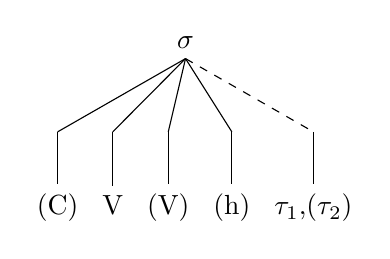
\begin{tikzpicture}
\Tree [.$\sigma$ 
          [\node[style={align=center}]{(C)};]
          [\node[style={align=center}]{V};]
          [\node[style={align=center}]{(V)};]
          [\node[style={align=center}]{(h)}; ]
          \edge[dashed];
          [\node[style={align=center}](tone){$\tau_1$,($\tau_2$)};]
        ]
\end{tikzpicture}
    \caption{Syllable Structure}
    \label{fig:syllstruc}
\end{figure}
\subsection{Types of syllable structure}
In the following section I will give examples for each type of syllable in the Hapi language, of which there are five different types, namely: V, CV, CVh, CVV and CVVh. 
Firstly, the simplest of all possible syllables is V. (\ref{Vex}) gives an example for this syllable type. 

\begin{columns}\label{Vex}
    \cols /à/ & [a˩] & \emh{à} & \textsc{link}
\end{columns}


This grammatical particle is depicted formally in figure (\ref{fig:Vex}).

\begin{figure}[H]
    \centering
    \begin{tikzpicture}[sibling distance=60pt]
        \Tree [.$\sigma$ 
                [.V
                \node[style={align=center}]{a};
                ]
               \edge[dashed]; [\node[style={align=center}]{$\tau=$L};]
                ]
    \end{tikzpicture}
    \caption{Syllable Structure: Example 1}
    \label{fig:Vex}
\end{figure}

Then, filling in the onset yields the next syllable type, CV. Example (\ref{CVex}) is an example for this syllable type.

\begin{columns}\label{CVex}
    \cols /kó/ & [ko˥] & \emh{kó} & 3\textsc{sm}
\end{columns}

The phonological form of this pronoun is depicted formally in figure \ref{fig:CVex}

\begin{figure}[H]
    \centering
    \begin{tikzpicture}[sibling distance=40pt]
        \Tree [.$\sigma$ 
                [.C
                \node[style={align=center}]{k};
                ]
                [.V
                \node[style={align=center}]{o};
                ]
               \edge[dashed]; [\node[style={align=center}]{$\tau=$H};]
                ]
    \end{tikzpicture}
    \caption{Syllable Structure: Example 2}
    \label{fig:CVex}
\end{figure}

We can now add another vowel to the nucleus, yielding a syllable of the type CVV and a new tone slot, as depicted in example (\ref{CVVex}) and figure \ref{fig:CVVex}.\footnote{Note that syllables of the type VV are also possible. The author has decided not to list this rarely occuring feature.}

\begin{columns}\label{CVVex}
    \cols /pói/ & [poi̯˥˧] & \emh{pói} & 2\textsc{s}
\end{columns}


\begin{figure}[H]
    \centering
    \begin{tikzpicture}[sibling distance=30pt]
        \Tree [.$\sigma$ 
                [.C
                \node[style={align=center}]{p};
                ]
                [.V
                \node[style={align=center}]{o};
                ]
                [.V
                \node[style={align=center}]{i};
                ]
               \edge[dashed]; [\node[style={align=center}]{$\tau=_1$H, $\tau_2=$M};]
                ]
    \end{tikzpicture}
    \caption{Syllable Structure: Example 3}
    \label{fig:CVVex}
\end{figure}

Now onto the last two syllable types: by filling in the coda with /h/, the syllable becomes closed, as can be seen in examples (\ref{CVhex}) and (\ref{CVVhex}) and in figures \ref{fig:CVhex} and 
\ref{fig:CVVhex}.

\begin{columns}\label{CVhex}
    \cols /sóh/ & [soh˥] & \emh{sóh} & `and, with'
\end{columns}

\begin{columns}\label{CVVhex}
    \cols /ʂòih/ & [ʂoi̯ʔ˩˧] & \emh{xòih} & `(my) brother'
\end{columns}




\begin{figure}[H]
    \centering
    \begin{tikzpicture}[sibling distance=30pt]
        \Tree [.$\sigma$ 
                [.C
                \node[style={align=center}]{s};
                ]
                [.V
                \node[style={align=center}]{o};
                ]
                [.h
                \node[style={align=center}]{h};
                ]
               \edge[dashed]; [\node[style={align=center}]{$\tau_1=$H, $\tau_2$=M};]
                ]
    \end{tikzpicture}
    \caption{Syllable Structure: Example 4}
    \label{fig:CVhex}
\end{figure}

\begin{figure}[H]
    \centering
    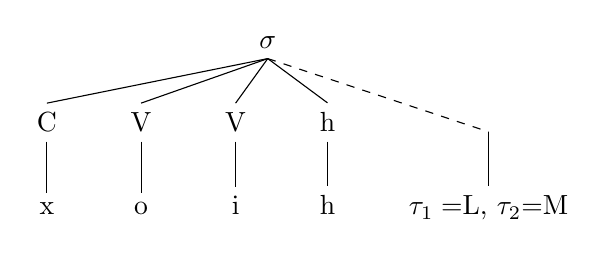
\begin{tikzpicture}[sibling distance=20pt]
        \Tree [.$\sigma$ 
                [.C
                \node[style={align=center}]{x};
                ]
                [.V
                \node[style={align=center}]{o};
                ]
                [.V
                \node[style={align=center}]{i};
                ]
                [.h
                \node[style={align=center}]{h};
                ]
               \edge[dashed]; [\node[style={align=center}]{$\tau_1=$L, $\tau_2$=M};]
                ]
    \end{tikzpicture}
    \caption{Syllable Structure: Example 5}
    \label{fig:CVVhex}
\end{figure}

\section{Tone}\label{stone}
In this section I will discuss the tonal system of Hapi. The language distinguishes three tones, the high tone, the neutral middle tone and the low tone. All tones may occur in any combination within the syllable and the phonological word. The tentative Hapi orthography marks tone using diacritics: the high tone is represented by the acute ◌́, the low tone is depicted by the grave diacritic ◌̀ and the middle tone is left unmarked.
Examples (\ref{tone1} - \ref{tone3}) present instances of each tone.

\begin{columns}\label{tone1}
    \cols /káiʂo/ & [kxai̯˥˧ʂo˧] & \emh{káixo} & `(my) mother'
\end{columns}

\begin{columns}
    \cols /ʂapati/ & [ʂa˧pa˧ti˧] & \emh{xapati} & `string (of a bow)'
\end{columns}

\begin{columns}\label{tone3}
    \cols /tàhòhì/ & [tʰa˩ho˩çi˩] & \emh{tàhòhì} & `poison (for a dart)'
\end{columns}

Tones may also be realized as floating tones on certain morphemes, e.g. the 'on top' suffix \emh{-(V̀)xa}. In these cases, the preceding vowel may take the floating tone, or the preceding tone is overwritten, as can be seen in example (\ref{tone4})


\begin{columns}\label{tone4}
    \cols /táíʂo/ & [tai̯˥ʂo˧] & \emh{táíxo} & `stave'
    \cols /táíʂòʂa/ & [tai̯˥ʂo˩ʂa˧] & \emh{táíxòxa} & `stave (on top)'
\end{columns}


\section{Morphophonology}\label{smorphophono}
In this section I will consider various morphophonological processes that occur in the Hapi language. To start, I will clarify the terms of some morphophonological units such as the conjunct affix, the disjunct affix and the clitic in section \ref{sunitdefinition}. I will present some allomorphic variations in section \ref{sallomorphicvariations} that apply to all morphemes with the required environment, then moving onward to discuss each morpheme that exhibits notable morphophonological changes towards its root in section \ref{morphophonomorphemespecific}. Doing that, I will begin with the plural marker \Pl, then moving on to the diminutive marker {\Dim} in the sections \ref{morphophonoplural} and \ref{morphophonodim}. Afterwards, I will consider the morphophonology of the declarative disjunct suffix {\Decl} in section \ref{sdeclassim}.
\subsection{Definitions of morphophonological Units}\label{sunitdefinition}
In the following section I will examine the definitions of the morphophonological units employed in the Hapi language,  namely, the conjunct affix, the disjunct affix, the clitic and the particle. 
\subsubsection{Conjunct Affixes}
In the Hapi language, those affixes are classified as conjunct affixes which do constitute a single phonological word unit with the stem and attach on stem-level. However, they do not change the stress distribution within the word, so that stress invariably falls on a syllable that belongs to the stem. In interlinear gloss, this type of morphemic juncture is denoted by `-', as can be inferred by example (\ref{ex:conjunctaffix}).
\begin{examples}
\ex \label{ex:conjunctaffix}
\script ˈtʰiː˧ʃi˥aʔ˥
\bits tiisí -áh
\gloss amulet {\Aug}
\tr the/a big (i.e. mighty) amulet
\end{examples}
\subsubsection{Disjunct Affixes}
While conjunct affixes attach to the stem and form a tight unit with it, disjunct affixes attach to the word unit on the word-level. However they're still more tightly bound to the phonological word as other words, as section \ref{smorphonodistinc} shows.  They do not change stress, and do not form a morphophonological unit with the word, so that rules like for example the debuccalization of /h/ at the end of a word apply to the affix-stem unit. In interlinear gloss, this type of juncture is marked by `=', as can be seen in example (\ref{ex:disjunctaffix}).\footnote{Note, that cross-linguistically, this sign is used to mark clitics; in this grammar however, `\texttt{==}' will be used to denote such phrase-level morphemes.}
\begin{examples}
\ex \label{ex:disjunctaffix}
\script ha˧ˈtaː˧˥çiʔ˧ko̯a˥˧
\bits ha- taápi -h =kóa
\gloss {\Antip} paint {\Ff} {\Decl}
\tr (I) am painting (something)
\end{examples}
\subsubsection{Clitics}
In Hapi grammar, clitics are morphemes which attach at phrase-level, i.e. cannot change stress but form a morphophonological unit with the word they attach to, whether it be the head or the dependent of a phrase. The clitic is marked by `\texttt{==}', and its usage is showcased in example (\ref{ex:clitic}).
\begin{examples}
\newbaarucmd{\cl}{\baarujuncture{\texttt{==}}}
\ex \label{ex:clitic}
\script ... ˈʃiː˥˧ti˧to˧
\bits tàhòhí -h kàah -xí =kóa síiti -∅ \cl to
\gloss poison {\Erg} kill {\Rpasto} {\Decl} uakari {\Abs} {\Vis}
\tr (Earlier today,) the poison (of a dart) killed an uakari monkey, I saw that
\end{examples}
\subsubsection{Distinction from Words and ʔ-Insertion}\label{smorphonodistinc}
While the distinction word-clitic, or especially the difference between word and disjunct might appear shallow at first, upon further introspection into the phonological processes that appear on word boundaries, the difference might become clearer.
The main process that plays a significant role in this is the so-called ʔ-Insertion on empty onsets. This is a process that exclusively applies on word-initial empty onsets, which are then filled with a glottal stop [ʔ]. In example (\ref{ex:gsinsert}), an example is given for \textbf{a)} glottal stop insertion, and \textbf{b)} a proof on how disjuncts are distinct from conjuncts, more specifically, how certain allophonic processes only occur within the phonological word. For the sake of simplicity, I will not transcribe tone in this example.
\begin{examples}
\newbaarulinetype{aligned}{ipa}{}
\newbaarulinetype{aligned}{ans}{}
\newbaarucmd[ans]{=}{\baarujuncture{\texttt{=}}}
    \ex \label{ex:gsinsert}
    \words tàhopoí tóti xàahaó\MC2 kaihatoo póóihaó\MC3 páikòih\MC3 kóhsa\MC2 ítàahaká\MC4 hìhohihákoo\MC2
    \ans S Adv V Disj Adv [[V Aff]ₚ Disj]ₛ [Aff N Aff]ₚ N ∅ [[Aff V Aff]ₚ Disj]ₛ [Disj [V]ₚ]ₛ 
    \ipa tʰa.ˈo.poi̯ ˈtʰo.ti χaː hao̯ kxai̯.ˈa.toː pʰoː.i ʔ hao̯ pʰai̯ koi̯ ʔ kxoh.sa {∅} ʔi taː ha ka çi.o.çi ˈso.to
    \bits tàhopoí tóti xàa =haó kaihatoo póói -h =haó pái- kòi -h kóhsa -∅ í- tàa -a =ká hìhohi= hákoo
    \gloss {\Fas}:{\Agent} ready {\Cop} \textsc{s/a>a(se)} now arrive {\Ff} \textsc{s/a>a(se)} {\Sshposs} house {\Dat} matter {\Abs} {\Intrg} {\Aux} {\Ff} {\Decl} delay {\Obligative}
    \tr Being ready, arriving at your house, should we (still) delay the affair?\footnote{In this example []ₚ indicates a phonological word, while []ₛ denotes the disjunct-word unit.}
\end{examples}
Processes like k→kx, t→tʰ and p→pʰ, which are widely spread throughout the phonological realm, appear only near word-boundaries (namely, on the beginning of a word), and not on disjunct boundaries. An example is given in (\ref{ex:morphodistinc1}) and (\ref{ex:morphodistinc2}).
\begin{examples}
    \newbaarulinetype{aligned}{ipa}{}
    \ex \label{ex:morphodistinc1}
    \script so.ˈsaː.i kxo
    \ipa so.ˈsaː.i kxo
    \bits sosáai kó
    \gloss cat {\Tsm}
    \tr tomcat
    \ex \label{ex:morphodistinc2}
    \script çi.ˈki.ʃiʔ.ko̯a
    \ipa çi ˈki.ʃiʔ ∅ ko̯a
    \bits hi- kísih -h =kóa
    \gloss {\Antip} dislike {\Ff} {\Decl} 
    \tr I dislike (it)
\end{examples}
\subsection{Allomorphic Variations}\label{sallomorphicvariations}
In this section I will discuss the basic parameters and morphophonological processes that apply to most, if not all bound morphemes in the Hapi language. The basic constraints or parameters of all bound morphemes are as follows. 
\subsubsection{Degemination of |h-h|}
Every context |h-h| is degeminated to |h|. This context is formalized in (\ref{ph:allom1}) and exemplified in (\ref{ex:ph:allom1}).
\begin{examples}
\ex \label{ph:allom1} \phon{h-h}{h}
\end{examples}
\begin{examples}
\ex\label{ex:ph:allom1}
\words sááí\MC2 háikia\MC2 kaai tà hóahkóa\MC3
\bits sáá =í háiki -a kaai tà hóah -h =kóa
\gloss eat \textsc{s/a>s(se)} type.of.nut {\Pl} foul {\Fs}:{\Subject} vomit {\Ff} {\Decl}
\tr After having eaten (some) foul nuts, I am (now) vomiting
\end{examples}
\subsubsection{Coalescence of morphemes in rapid speech}
Certain morphemes are fused in rapid speech, however there haven't been made any observations about these coalescence patterns. An example is given in (\ref{ex:rapidspeech}).
\begin{examples}
\ex \label{ex:rapidspeech}
\manner rapid speech
\words kaóxììhaíh\MC2 kíih hóíaka\MC3 xáháìh\MC2 xíoki
\bits kaóxììha -íh kíih hóí -a =ka xáháìi -h xíooki
\gloss teacher {\Erg} old give {\St} {\Decl} student {\Dat} gift
\tr The old teacher gives a gift to a student
\end{examples}
\subsubsection{/h/-Insertion}
In each context of the form |VV-V|, /h/ is inserted on the morpheme boundary. This process is schematized in (\ref{ph:hinsert}) and exemplified in (\ref{ex:ph:hinsert}). In the context |V-VV| the same rule applies.
\begin{examples}
\ex \label{ph:hinsert} \phon{VV-V}{VVhV}
\ex \label{ex:ph:hinsert}
This section is work-in-progress
\end{examples}
\subsection{Morpheme-specific Processes}\label{morphophonomorphemespecific}
\subsubsection{Debuccalization of the marker \texorpdfstring{\Pl}{PL}}\label{morphophonoplural}
The debuccalization of the abbreviated version of the plural marker \Pl, namely the morpheme \emh{-s} is one of the most widely appearing processes in the Hapi language. The rule can be formalized as presented in (\ref{ph:plurals}). An instance of this process is exemplified in (\ref{ex:ph:plurals}).
\begin{examples}
\ex \label{ph:plurals} \phonr{s}{h}{C}
\ex \label{ex:ph:plurals}
\words ókoíhtah\MC4
\bits ó- koí -s -tah
\gloss {\Ssposs} hut {\Pl} {\Prl}
\tr (we shall go) via your huts
\end{examples}
\subsubsection{The Diminutive marker \texorpdfstring{\Dim}{DIM}}\label{morphophonodim}
The diminutive marker \textsc{dim} undergoes two major processes: firstly, the deletion of the morpheme's onset, secondly, the dissimilation of the morpheme's nucleus. The deletion of the morpheme's onset, namely, of |ʂ|, appears in the context of a preceding /h/; this rule is formalized in (\ref{ph:dim}), an example is given in (\ref{ex:dim1}), but shall be reiterated here. 
\begin{examples}
\ex \label{ph:dim} \phonl{ʂ}{∅}{h}
\ex \label{ex:ph:dim}
\words hápaahii\MC2
\bits hápaah -xii
\gloss dog {\Dim}
\tr the little dog
\end{examples}
The dissimilation of the morpheme's nucleus happens in the context of an /i/ in the preceding syllable's nucleus. This rule is depicted in (\ref{ph:dim2}) and exemplified in (\ref{ex:ph:dim2}).
\begin{examples}
\ex \label{ph:dim2} \phonl{iː}{o}{i(h).C}
\ex \label{ex:ph:dim2} 
\words hósiixo\MC2
\bits hósii -xii
\gloss son {\Dim} 
\tr the/a grandson
\end{examples}
\subsubsection{Assimilation of the declarative affix \texorpdfstring{\Decl}{DECL}}\label{sdeclassim}
The declarative disjunct affix \Decl, \emh{=kóa}, is often reduced to \emh{=ká} or \emh{=ka} after a syllable containing /a/. This context is formalized in (\ref{ph:decl}) and an example is given in (\ref{ex:ph:decl}).
\begin{examples}
\ex \label{ph:decl} \phonl{kóa}{ka,ká}{a}
\ex \label{ex:ph:decl}
\words kó hásaaka\MC3 taahsáahi\MC2
\bits kó hásaa -a =kóa taah -sáahi
\gloss {\Tsm}:{\Subject} be.the.first {\St} {\Decl} effort {\Pvt}
\tr He won (the race) without any effort
\end{examples}
\chapter{The Noun and the Noun Phrase}
This chapter discusses the noun and the noun phrase in the Hapi language. In the first section of this chapter, I will present the nominal morphology of the language. I will start by considering the nominal root and the noun structure in section \ref{snomroot}, then discussing gender marking in \ref{sgender}. I will move on and present the number marking, as well as diminutives and augmentatives in the sections \ref{snumber}, \ref{sdim} and \ref{saug}. In section \ref{spossession} I will consider the language's possessive system, first covering possessable, and then unpossessable nouns. In section \ref{scase} I will discuss the Hapi case system in all its complexity.
Moving onward onto section \ref{snounphrase} I will consider the structure of the noun phrase and its components, starting with the order of the noun phrase elements in \ref{snounorder} and an overview of the Hapi pronoun system in section \ref{spronouns}. After a comprehensive consideration of the language's classifier system in \ref{sclassifier}, I will lay out the different parts of the noun phrase in the sections \ref{sdemonstrative}, \ref{squantifier} and \ref{sattributes}.

\section{Nominal Morphology}
The internal structure of Hapi nouns is examined in this section, focussing on the grammatical categories encoded by nominal morphology i.e. gender, number, diminutives, augmentatives, possession and case.
\subsection{Nominal Root}\label{snomroot}
The structural properties of the nominal root include a set of suffixes responsible for the expression of number, diminutives, augmentatives, and case, while a set of prefixes is used to express possession on possessable nouns. Nominal roots can be divided into two morphophonological subtypes, which take different prefixes depending on the first segment in the root. If \textbf{(i)} the root starts with a vowel, then a certain set of prefixes is used, and if \textbf{(ii)} the root starts with a consonantal sound, another set is employed. 
\subsubsection{Internal structure of nominal roots}
% 17 mono, 67 disyllabic, 26 trisyllabic, 3 polysyllabic → 113 roots

In the following section I will consider the internal phonological structure of nominal roots, starting with the rare monosyllabic roots, then moving onward to the comparatively often found disyllabic, trisyllabic and polysyllabic, i.e. roots with more than four syllables, roots.
\paragraph{Monosyllabic roots}
There is a set of \textit{17} monosyllabic roots in the Hapi language, which are all considered to be very basic roots. There have been no reports of roots of the structure V and CV. Some examples for monosyllabic roots of the shape CV, CVh, CVV and CVVh are given in example (\ref{nomroot1ex}), (\ref{nomroot2ex}) and (\ref{nomroot3ex}).

\begin{columns}\label{nomroot1ex}
    \cols  /ʂòih/ & [ʂoi̯ʔ˩˧] & \emh{xòih} & `(my) brother'
\end{columns}
\begin{columns}\label{nomroot2ex}
    \cols  /píː/ & [çiː˥] & \emh{píí} & `major river'
\end{columns}
\begin{columns}\label{nomroot3ex}
    \cols  /kóih/ & [kxoi̯ʔ˥˧] & \emh{kóih} & `hideout'
\end{columns}


\paragraph{Disyllabic roots}
The majority of nominal roots in the Hapi language are disyllabic. In the analyzed corpus of \textit{113} nominal roots, there were \textit{67} disyllabic roots. 
\paragraph{Trisyllabic and polysyllabic roots}
There is a decent amount of tri- and polsyllabic nominal roots in the Hapi language. Trisyllabic roots are mostly of the shape CV.CV.CV, CV.CV.CVV, CV.CV.VV and CV.CVV.CV. Some examples for tri- and polysyllabic nominal roots are given in example (\ref{nomroot4ex}) - (\ref{nomroot6ex}).

\begin{columns}\label{nomroot4ex}
    \cols /hòkaapa/ & [ho˩kxaː˧pa˧] & \emh{hòkaapa} & `hunter'
\end{columns}
\begin{columns}\label{nomroot5ex}
    \cols /papáʂi/ & [pʰa˧pa˥hi˧] & \emh{papáxi} & `door'
\end{columns}
\begin{columns}\label{nomroot6ex}
    \cols /háhopìi/ & [ha˥oçiː˩˧] & \emh{hahópìi} & `sloth'
\end{columns}

\subsubsection{Overview}
An overview of the nominal stem structure of the Hapi language can be seen in table \ref{nstruco}.
In the first prefix slot, the possessive markers can be found, right before the root. Then, the augmentative and diminutive conjunct suffixes are placed right after the root. The case markers are located afterwards, only being interrupted by the number marker \emh{-(so)a}.
\begin{table}[p!]
    \centering
    \Rotatebox{90}{%
    \begin{tabular}{@{}ccccccclc@{}}
    \toprule
    \multicolumn{4}{c}{-1} & 0 & 1 & 2 & \multicolumn{1}{c}{3} & 4 \\ \midrule
    \multicolumn{4}{c}{Possession} & ROOT & Aug/Dim & Case & \multicolumn{1}{c}{Number} & Case \\ \midrule
     &  & \#V & \#C & \multirow{8}{*}{} & AUG & \multirow{8}{*}{see Section 4.1.7} & \multicolumn{1}{c}{PL} & \multirow{8}{*}{see Section 4.1.7} \\ \cmidrule(r){1-4} \cmidrule(lr){6-6} \cmidrule(lr){8-8}
    \multirow{2}{*}{1} & SG & \multirow{2}{*}{h́-} & há- &  & -áh- / -aóh- &  & \multicolumn{1}{c}{-(so)a} &  \\ \cmidrule(lr){2-2}
     & PL &  & hi- &  & DIM &  & \multicolumn{1}{c}{} &  \\ \cmidrule(lr){2-2} \cmidrule(lr){6-6}
    2 & SG & \multicolumn{2}{c}{ó-} &  & -xii- &  &  &  \\ \cmidrule(lr){2-2}
     & PL & oh- & o- &  & \multicolumn{1}{l}{\multirow{4}{*}{}} &  &  &  \\ \cmidrule(lr){2-2}
     & HON & pò- & pái- &  & \multicolumn{1}{l}{} &  &  &  \\ \cmidrule(lr){2-2}
    3 & SG & k̀- & kì- &  & \multicolumn{1}{l}{} &  &  &  \\ \cmidrule(lr){2-2}
     & PL & t̀- & tà- &  & \multicolumn{1}{l}{} &  &  &  \\ \bottomrule
    \end{tabular}}
    \caption{Nominal Stem Structure}
    \label{nstruco}
\end{table}

\subsection{Gender}\label{sgender}
While gender is not explicitly marked on nouns, it can be denoted by using a noun and the respective third person female or male pronoun, namely \emh{hoa} and \emh{kó}, juxtaposing it after the inflected noun root, as can be seen in examples (\ref{nomgender1}) and (\ref{nomgender2}).
\begin{example}
\label{nomgender1}
\bits hàòxa hoa
\gloss capybara {\Tsf}
\tr female capybara
\end{example}
\begin{example}
\label{nomgender2}
\bits hàòxa kó 
\gloss capybara {\Tsm} 
\tr male capybara
\end{example}
\subsection{Number}\label{snumber}
The Hapi language distinguishes two types of number marking on nouns, singular and plural, glossed as {\Sg} and {\Pl} respectively. While the singular is left unmarked, the plural is marked by the suffix \emh{-(so)a}, as can be seen in examples (\ref{ex:number1}) and (\ref{ex:number2}). Instead of the full form \emh{-soa}, the abbreviated form \emh{-s} may be used, as exemplified in (\ref{ex:number3}).\footnote{In this case the abbreviated plural marker \emh{-s} is morphophonologically debuccalized to /h/.}
\begin{examples}
\ex
\label{ex:number1}
\bits há- sáhpa -soa
\gloss {\Fsposs} arrow.head {\Pl}
\tr my arrowheads; my collection of arrowheads
\ex
\label{ex:number2}
\bits hóh -áh -a -óh
\gloss man {\Aug} {\Pl} {\Erg}
\tr (the) big men (had slain a snake...)
\ex 
\label{ex:number3}
\bits ó- koí -s -tah
\gloss {\Ssposs} hut {\Pl} {\Prl}
\tr (we shall go) via your huts
\end{examples}
\subsection{Diminutives}\label{sdim}
To form a noun's diminutive form, the suffix \emh{-xii} is used. It cannot only used be for simple diminutives as in (\ref{ex:dim1}), but also is employed derivationally for certain noun>noun processes; for example, it may be used for the derivation of `grandson' from the word `son', or can be used pejoratively to derive nouns that are connotated with a certain derogatory sense, as in (\ref{ex:dim2}) and (\ref{ex:dim3}).
\begin{examples}
\ex
\label{ex:dim1}
\bits hápaah -xii 
\gloss dog {\Dim}
\tr the little dog
\ex
\label{ex:dim2}
\bits pái- hósii -xii
\gloss {\Sshposs} son {\Dim}
\tr your\textsubscript{HON} grandson
\ex
\label{ex:dim3}
\bits páhsóoih -a -xii
\gloss bug {\Pl} {\Dim}
\tr those pesky little bugs!
\end{examples}
\subsection{Augmentatives}\label{saug}
The augmentative form, which is marked by the suffix \emh{-áh} \Aug, encodes augmentative semantics, as well as derives kinship terms in the opposite direction as the diminutive, i.e. \emh{káixo} `mother' > \emh{káixoáh} `grandmother', as exemplified in (\ref{ex:aug1}) and (\ref{ex:aug2}). It may also encode some sort of honorific sense of praising, as can be seen in example (\ref{ex:aug3}).
\begin{examples}
\ex
\label{ex:aug1}
\bits táhaa -áh 
\gloss barrel {\Aug}
\tr a big barrel
\ex
\label{ex:aug2}
\bits kápihoo -áh
\gloss father {\Aug}
\tr (my) grandfather
\ex
\label{ex:aug3}
\bits hahópìi -áh
\gloss sloth {\Aug}
\tr (Praise be!) The sloth god!
\end{examples}
There is also the augmentative suffix \emh{-aóh}, which may be employed in the same sense as \emh{-áh} \Aug. (\ref{ex:aug4}) gives an example for an augmentative using the second augmentative suffix.
\begin{examples}
\ex 
\label{ex:aug4} 
\bits ahitáh -aóh
\gloss iguana {\Auga}
\tr a huge iguana
\end{examples}
The two augmentative suffixes may also be stacked to increase the augmentative, praising meaning usually encoded by these morphemes. In this case, the suffix \emh{-áh} comes first, as can be seen in example (\ref{ex:aug5}).
\begin{examples}
\ex
\label{ex:aug5}
\bits sósikíí -áh -aóh
\gloss wooden.beam {\Aug} {\Auga}
\tr an immense wooden beam
\end{examples}
\subsection{Possession}\label{spossession}
There are several types of possession in the Hapi language, which are presented in the following section. I will consider possessable nouns in section \ref{salien} and will discuss unpossessable nouns in section \ref{sinalien}. Concerning the different types of possession, an overview is given in this section. The Hapi language distinguishes between \textbf{(i)} possessable and \textbf{(ii)} unpossessable nouns. Unpossessable nouns can further be subdivided into \textbf{(iia)} indirect possessesable unpossessable nouns and \textbf{(iib)} inherently possessed unposessable nouns. 
\subsubsection{Possessable Nouns}\label{salien}
Most nouns in the language are possessable, i.e. can be marked for possession by the employment of personal markers which are prefixed to the root. I will discuss the employment of personal markers in \ref{spossmarker} and the interaction between possession and nominal classifier, discussing a construction called the possesive classifier construction in section \ref{snomclassifiersandpossession}
\paragraph{Personal Markers}\label{spossmarker}
There are personal marker which may be employed to encode possession on possessable nominals. Table \ref{tpossmarker} gives an overview of the personal marker paradigm.
\begin{table}[H]
\centering
\begin{tabular}{@{}cccc@{}}
\toprule
\multicolumn{2}{c}{\multirow{2}{*}{Person}} & \multicolumn{2}{c}{Morpheme} \\ \cmidrule(l){3-4} 
\multicolumn{2}{c}{} & \#V & \#C \\ \midrule
1 & SG & \multirow{2}{*}{h́-} & há- \\ \cmidrule(lr){2-2}
 & PL &  & hi- \\ \cmidrule(lr){2-2}
2 & SG & \multicolumn{2}{c}{ó-} \\ \cmidrule(lr){2-2}
 & PL & oh- & o- \\ \cmidrule(lr){2-2}
 & HON & pò- & pái- \\ \cmidrule(lr){2-2}
3 & SG & k̀- & kì- \\ \cmidrule(lr){2-2}
 & PL & t̀& tà- \\ \bottomrule
\end{tabular}
\caption{Possessive personal markers: Overview}
\label{tpossmarker}
\end{table}
Some examples for the usage of these personal markers can be found below. Example (\ref{ex:poss1}) and (\ref{ex:poss2}) showcase the employment of the '\#V floating tone' markers \emh{h́-} and \emh{t̀-}, while (\ref{ex:poss3}) exemplifies the usage of the honorific marker \emh{pái-}. As can be seen in example (\ref{ex:poss2}), the third person plural morpheme may also be used as an inter-clausal forth person pronoun. This is true for most employments of this pronoun, not only in its possessive form.
\begin{examples}
\ex
\label{ex:poss1}
\words háhoáta\MC2
\bits h́- ahoáta
\gloss {\Fsposs} bow
\tr my/our bow
\ex
\label{ex:poss2}
\words tàhoáta\MC2
\bits t̀- ahoáta
\gloss {\Tpposs} bow
\tr their bow/hisⱼ bow
\ex 
\label{ex:poss3}
\words páipáaxo\MC2
\bits pái- páaxo
\gloss {\Sshposs} tendon
\tr your\textsubscript{HON} tendon (the one you extracted from the meat)
\end{examples}
\paragraph{Nominal Classifiers and Possession}\label{snomclassifiersandpossession}
There is also another special construction to express possession, using nominal classifiers and personal markers. This constructions is showcased in example (\ref{ex:poss4}). After the inflected noun, the according classifier is inserted, with the respective personal marker attached to it.\footnote{More on nominal classifiers in section \ref{sclassifier}} 
The classifier may also be moved to the front within a clause to focus the aspect of possession, as can be seen in example (\ref{ex:poss5}).
\begin{examples}
\ex
\label{ex:poss4}
\bits káhi kì- hóó
\gloss chicken.egg {\Tsposs} {\Cl}:egg  
\tr his chicken egg
\ex
\label{ex:poss5}
\words hóhóikaííxi\MC2 kói\MC2 hò\MC2 póóihi\MC2 xósóóxíkóa\MC4 hápaáh\MC2
\bits {hó$\sim$ hóika} =ííxi koí -∅ h- ò póói -i xósóó -xí -∅ =kóa hápaáh -h 
\gloss {\Redup}:build \textsc{s/a/o>o(se)} hut {\Abs} {\Fsposs} {\Cl}:anim:sg come {\Dep} bite {\Rpasto} {\St} {\Decl} dog {\Erg} 
\tr As he was once again building another hut, my dog came and bit (him)
\end{examples}
\subsubsection{Unpossessable Nouns}\label{sinalien}
There is a closed set of unpossessable nouns in the Hapi language, which either \textbf{(i)} can't be possessed directly, or \textbf{(ii)} can't be possessed at all, with a suppletive, possessable form being used for other means of possession. Those two types are called indirect possessable unpossessable nouns and inherently possessed unpossessable nouns. I will first consider indirect possessable unpossessable nouns in this section, just before presenting the different semantic aspects of inherently possessed unpossessable nouns, as well as showcase their suppletive possessable forms. 
The semantics of indirect possessable unpossessable nouns (henceforth indPUNs; c.f. inherently possessed unpossessable nouns, inhPUNs) vary greatly within the language, and are summarized in table \ref{t:ccsgip}, where an overview of the most common cross-linguistic semantic groups in Hapi is given.
\begin{table}[H]
\centering
\captionsetup{justification=centering}
\begin{tabular}{@{}lll@{}}
\toprule
Semantic Group & Example & Possessability \\ \midrule
landscape features & rivers, mountains & indPUN \\
professions & hunters, shamans & indPUN \\
social relationships & neighbour, servant & indPUN \\
kinship terms & mother, brother & inhPUN \\
body parts & head, limbs & inhPUN \\
possessive attributes & age, name & inhPUN \\
mental states & fear, mind & (possessable) \\
part-whole relationships & side, top & (possessable) \\ \bottomrule
\end{tabular}
\caption{Common Cross-linguistic Semantic Groups and their Possessability in Hapi}
\label{t:ccsgip}
\end{table}
IndPUNs include geographical features, such as rivers, mountains or trees, as well as professions or persons, such as hunters and shamans. 
They all may be possessed via certain indirect possession strategies which are showcased in examples (\ref{ex:poss6}), (\ref{ex:poss7}) and (\ref{ex:poss8}). In these cases, the possession is semantically quite indirect, only encoding loose association, e.g. proximal distance to landscape features or the belonging to a family of professions and persons. 
\begin{examples}
\ex 
\label{ex:poss6}
\bits hòkaapa hi- táa
\gloss hunting.person {\Fpposs} {\Cl}:profession
\tr our hunter; the hunter that belongs to our family
\ex
\label{ex:poss7}
\bits xííkoh =à tàahoih
\gloss hill {\Link} {\Ff}
\tr my/our hill; the hill that is located near my/our hut
\ex
\label{ex:poss8}
\bits àkóóih xáa pòih
\gloss in.law {\Cop} {\Ss}.{\Dat}
\tr your in-law
\end{examples}
In example (\ref{ex:poss6}), the construction explained in section \ref{snomclassifiersandpossession} is employed; this construction is not only used in these cases, but also, as explained in the referred section, to focus the possessed noun. In example (\ref{ex:poss7}), another construction is used. The linking disjunct affix \emh{=à} is suffixed to the head, while the respective emphatic pronoun form is inserted right after it.\footnote{Compare section \ref{spronouns} for a comprehensive overview of the Hapi pronoun system.}
In example (\ref{ex:poss8}), the copula is used to connect the head noun with the dative form of the possessing pronoun. This construction is rather sparsely used, while the other ones are employed quite often. 
\paragraph{Kinship Terms}
Kinship terms are one of the most often used inhPUNs in the Hapi language. As they're all inherently possessed by the first person singular, they each have a suppletive form that can be regularly possessed using the prefixes discussed in section \ref{spossmarker}. Table \ref{t:kinship} gives an overview of the most commonly used kinship inhPUNs and their suppletive possessable counterparts. 
\begin{table}[H]
\centering
\begin{tabular}{@{}lll@{}}
\toprule
inhPUN & Possessable Form & Meaning \\ \midrule
xòih & kàháa & (my) brother \\
kápihoo & káota & (my) father \\
haóxí & hósii & (my) son \\
káixo & xapisóo & (my) mother \\ \bottomrule
\end{tabular}
\caption{InhPUNs and Suppletive Forms (Kinship)}
\label{t:kinship}
\end{table}
Example (\ref{ex:poss9}), (\ref{ex:poss10}) and (\ref{ex:poss11}) showcase the usage of the suppletive forms. 
\begin{examples}
\ex
\label{ex:poss9}
\bits tài xàa haóxí -ò
\gloss {\Dem}:{\Prox} {\Cop} son {\Cl}:anim:sg
\tr This is my son
\ex
\label{ex:poss10}
\bits:* tài xàa ó- haóxí -ò
\gloss {\Dem}:{\Prox} {\Cop} {\Ssposs} son {\Cl}:anim:sg
\intended This is your son
\ex
\label{ex:poss11}
\bits tài xàa ó- hósii -ò
\gloss {\Dem}:{\Prox} {\Cop} {\Ssposs} son {\Cl}:anim:sg
\tr This is your son
\end{examples}
\subsection{Case}\label{scase}
In this section I will consider the language's case system. The Hapi case system is relatively complex, featuring a total of 10 cases, which can be subdivided into 3 core cases, 4 non-core cases and 3 relational cases. In section \ref{scorecase} I will discuss the language's core cases, in section \ref{sncorecase} I will present its non-core cases and in section \ref{srelcase} I will consider its relational cases.
\subsubsection{Core Cases}\label{scorecase}
In the following section I will present the language's core cases. These cases are employed to mark core arguments such as S, A, P, D, T, and R for their appropriate role. In this context, the absolutive case marks the S of intransitive verbs, as well as the P of transitive and the T of ditransitive verbs. The ergative case marks the A of transitive verbs and the D of ditransitive verbs, while the dative case marks most commonly the R of a ditransitive verb, but also the second argument of a extended intransitive clause.\footnote{See section \ref{s:verbclass} for more information on extended intransitive clauses.} These cases are all marked in the first case slot.
\paragraph{Absolutive Case \emh{-∅} \textsc{abs}}
Employed to encode the S of intransitive clauses, the primary function of the absolutive case is showcased in example (\ref{ex:abs1}); the speaker informs the listener about an extraordinary warrior, who, earlier on that day, showed mercy for an enemy warrior. This is seen as a very unusual and strange action to be done by a warrior, hence the explicit statement of the fact. 
\begin{examples}
\ex \label{ex:abs1}
\words toíhoh\MC2 sáhaaxíkóa\MC4
\bits toíhoh -∅ sáhaa -xí -∅ =kóa 
\gloss warrior {\Abs} show.mercy {\Rpasto} {\St}  {\Decl} 
\tr Earlier today, the warrior showed mercy
\end{examples}
Besides that, the absolutive case also marks the P of transitive clauses as in (\ref{ex:abs2}) and the T of ditransitive verb, thus making the Hapi language a indirective language. Example (\ref{ex:abs3}) gives an example for this tertiary function of the absolutive case.
In (\ref{ex:abs2}), the speaker talks about a young girl who ate an underripe mangaba fruit, and got stomach aches from it the day after. In (\ref{ex:abs3}), the speaker reports of a benevolent teacher, who gifts a student of his a present.
\begin{examples}
\ex \label{ex:abs2}
\words hoa sááhikóa\MC4 háiikáh\MC2
\bits hoa sáá -hi -∅ =kóa háiikáh -∅ 
\gloss {\Tsf}:{\Agent} eat {\Rpastt} {\St} {\Decl} type.of.fruit {\Abs}
\tr She ate a mangaba fruit (yesterday)
\ex \label{ex:abs3}
\words kaósóaíh\MC2 kíih hóíakóa\MC3 xáháìih\MC2 xíooki\MC2
\bits kaósóa -íh kíih hóí -a =kóa xáháìi -h xíooki -∅
\gloss teacher {\Erg} old give {\St} {\Decl} student {\Dat} gift {\Abs}
\tr The old teacher gives a gift to a student
\end{examples}
\paragraph{Ergative Case \emh{-(V́)h} \textsc{erg}}
This case is used to mark the A of transitive clauses, as well as the D of ditransitive verbs. These two functions are exemplified in (\ref{ex:erg1}) and (\ref{ex:abs3}).
In (\ref{ex:erg1}), the neighbour of the speaker was taking the raw meat back from the fire place back to his hut, and this for unknown reasons.
\begin{examples}
\ex \label{ex:erg1}
\words àkóóihíh\MC2 xáh hóhiaka\MC3
\bits àkóóih -íh xáh hóhi -a =kóa 
\gloss  neighbour {\Erg} raw.meat take {\St} {\Decl} 
\tr (My) neighbour is taking the raw meat (with him)
\end{examples}
\paragraph{Dative Case \emh{-V̀Vh/-s} \textsc{dat}}
The dative case is used to mark the R of a ditransitive clause, as well as the extended argument of an extended intransitive clause. These two contexts are exemplified in (\ref{ex:abs3}) and (\ref{ex:dat1}). In (\ref{ex:dat1}), a child is playing with the mud.
\begin{examples}
\ex \label{ex:dat1}
\words kó sahóóhakóa\MC3 xóahasàxa\MC3
\bits kó sahóó -a =kóa xóaha -s -àxa
\gloss {\Tsm}:{\Subject} carve.in {\St} {\Decl} mud {\Dat} {\Ont}
\tr He is scratching (something) in the mud
\end{examples}
\subsubsection{Non-Core Cases}\label{sncorecase}
The non-core cases are employed in the contexts of peripheral, non-core arguments, hence their name. There are four non-core cases, all of which are marked in the first case slot.
\paragraph{Locative Case \emh{-hóo} \textsc{loc}}
The locative case marks a noun for a locational meaning, i.e. the position in, from, or toward a certain object. Specifically, the locative case may bear a pure locational meaning, usually translated as `in, at', a lative meaning, which can be translated using the adposition `to(wards)', and an ablative meaning, i.e. `from, by'. These meanings are showcased in the examples (\ref{ex:loc1}), (\ref{ex:loc2}) and (\ref{ex:loc3}). In each of those, the speaker was asked to describe several contexts in which the verbs `be at', `go' and `come' were all used with the locative case. 
\begin{examples}
\ex \label{ex:loc1}
\words tàhokó hoihkóa\MC3 há pííháhóo\MC3
\bits tàhokó hoi -h =kóa há píí -áh -hóo
\gloss {\Fat}:{\Subject} be.at {\Ff} {\Decl} {\Cngr} river {\Aug} {\Loc}
\tr We(excl.) are at the river
\ex \label{ex:loc2}
\words tàhokó háahkóa\MC3 há pííháhóo\MC3
\bits tàhokó háa -h =kóa há píí -áh -hóo
\gloss {\Fat}:{\Subject} go {\Ff} {\Decl} {\Cngr} river {\Aug} {\Loc}
\tr We(excl.) go to the river
\ex \label{ex:loc3}
\words tàhokó póóihkóa\MC3 há pííháhóo\MC3
\bits tàhokó póói -h =kóa há píí -áh -hóo
\gloss {\Fat}:{\Subject} come {\Ff} {\Decl} {\Cngr} river {\Aug} {\Loc}
\tr We(excl.) come from the river
\end{examples}
\paragraph{Perlative Case \emh{-tah} \textsc{prl}}
The perlative case expresses that something is moved `through' or `along' the referent of the noun that is marked. It also marks the demoted A of passive constructions. The examples (\ref{ex:perl1}) and (\ref{ex:perl2}) demonstrate the case's usage. While (\ref{ex:perl1}) might not need any further explanation, (\ref{ex:perl2}) does. There, the speaker tells a narrative of a foolish young girl, who, at the end of the story, is eaten by a giant crab. This is a symbol for the punishment for her `unlawful' actions.
\begin{examples}
\newbaarucmd{\cl}{\baarujuncture{\texttt{==}}}
\ex \label{ex:perl1}
\words tàahopí há hááháah\MC3 ókoíhtah\MC4
\bits tàahopí há háá- háa -h  \\ ó- koí -s -tah 
\gloss {\Fas}:{\Subject} {\Cngr} {\Hort} go {\Ff} {\Ssposs} hut {\Pl} {\Prl}
\tr We shall go via your huts
\ex \label{ex:perl2}
\words hoó asááhàòkóapò\MC5 xáohaóhtah\MC3
\bits hoó a- sáá -hàò =kóa \cl pò xáoh -aóh -tah
\gloss {\Tsf}:{\Patient} {\Pass} eat {\Dpasto} {\Decl} {\Infer} crab {\Auga} {\Prl}
\tr She was eaten by a huge crab (they told me)
\end{examples}
\paragraph{Privative Case \emh{-sáahi} \textsc{pvt}}
The privative case expresses the acting of a verb `without' a certain noun, more or less yielding a construction of a `\textsc{noun}-less' meaning. Together with the copula marker \textit{xàa}, the semantics of `to not have \textsc{noun}' may be achieved. This and the more general meaning of the privative case are shown in examples (\ref{ex:pvt2}) and (\ref{ex:pvt1}). (\ref{ex:pvt1}) tells us about a young, inexperienced hunter who doesn't quite know how to separate meat from fat elegantly. In (\ref{ex:pvt2}), the speaker utters this sentence in the context of a hunt, in which another hunter has slain a green iguana, whereas the speaker has not.
\begin{examples}
\ex \label{ex:pvt1}
\words kó sahóóhikóa\MC3 tíahsáahi\MC2
\bits kó sahóó -hi =kóa \\ tíah -sáahi
\gloss {\Tsm}:{\Subject} separate.meat.from.fat {\Rpastt} {\Decl} care {\Pvt}
\tr He separated meat from fat carelessly
\ex \label{ex:pvt2}
\words ahitáhsáahi\MC2 xàa tà
\bits ahitáh -sáahi xàa tà
\gloss green.iguana {\Pvt} {\Cop} {\Fs}
\tr (Unlike you,) I do not have a green iguana
\end{examples}
\paragraph{Semblative Case \emh{-haixá} \textsc{smb}}
The semblative case denotes the similarity of the subject to the marked noun. This function is explained in example (\ref{ex:smb1}). There, the speaker narrates an event from his childhood, in which a sick stranger arrived at the village; his condition is described in (\ref{ex:smb1}).
\begin{examples}
\ex \label{ex:smb1}
\words haxápií hóahtóhikóa\MC3 tísoohaixá\MC2
\bits haxápií hóah -tóhi =kóa tísooh -haixá
\gloss stranger vomit {\Dpasto} {\Decl} frog {\Smb} 
\tr The stranger vomited like a frog
\end{examples}
\subsubsection{Relational Cases}\label{srelcase}
In this section I will consider the relational cases of the Hapi language. These cases are employed to specify a certain relational sense, i.e. they mark a noun for their spatial relationship with another noun. As will be discussed in section \ref{scasestacking}, these cases may be stacked with other non-core cases to yield more specified semantics. These cases are simply named after their English semantic equivalents;
\paragraph{`on top of' \emh{-(V̀)xa} \textsc{on.top} }
The `on top of' case primarily\footnote{Another usage is sketched out in section \ref{s:trans}} marks a noun's position to be roughly `on top of' another noun, as can be seen in example (\ref{ex:ontop1}). (\ref{ex:ontop2}) shows, how a construction of the shape `x-\textsc{on.top} y' can indicate possession in the form of `y has x'.
\begin{examples}
\ex \label{ex:ontop1}
\words haípi haahakóa\MC3 píihàxa\MC2
\bits haípi haah -a =kóa píihà -xa
\gloss soup cook {\St} {\Decl} fire.place {\Ont}
\tr The soup is cooking above the fire place
\ex \label{ex:ontop2}
\words kihaòhxa\MC2 póxihoo
\bits kihaòh -xa póxihoo
\gloss type.of.fruit {\Ont} {\Ss}
\tr You/youₚₗ have a tucumã fruit
\end{examples}
\paragraph{`below' \emh{-(t)aó} \textsc{below}}
The `below' case marks a noun's position to be roughly `below' another noun, as can be seen in example (\ref{ex:below1}).
\begin{examples}
\ex \label{ex:below1}
\words tàhòhì tísooh hoí xasíítaó\MC2
\bits tàhòhì tísooh hoí xasíí -taó
\gloss poison frog {\Cop} leaf {\Bel}
\tr The poison dart frog sits under the leaf
\end{examples}
\paragraph{`next to' \emh{-(h)aí} \textsc{next.to}}
The `next to' case marks a noun's position to be roughly `next to' another noun, as can be seen in example (\ref{ex:nextto1}). There, the speaker reports of a girl that was, defying the traditional Hapi culture, eating a soup next to her father, even though said traditions don't allow members of either gender to eat in the proximity of each other.
\begin{examples}
\ex \label{ex:nextto1}
\words pihih tááhtóhikóa\MC3 haípi kìkáotahaí\MC3
\bits pihih tááh -tóhi =kóa haípi kì- káota -haí
\gloss girl drink {\Dpasto} {\Decl} soup {\Tsposs} father {\Next}
\tr The girl was drinking soup next to her father
\end{examples}
\subsubsection{Case
Stacking}\label{scasestacking}
In the Hapi language, second slot cases may be stacked with first slot cases to yield specific semantics, which are shown in table \ref{t:casestacking}. Note that the privative and semblative cases do not allow any relational combination.
\begin{table}[H]
\begin{tabular}{@{}ccccc@{}}
\toprule
\multirow{2}{*}{} & \multicolumn{3}{c}{Locative}                        & \multirow{2}{*}{Perlative} \\ \cmidrule(lr){2-4}
                  & Locational        & Lative         & Ablative       &                            \\ \midrule
'on top of'       & focal 'on top of' & 'to above'     & 'from above'   & 'via above'                \\
'below'           & foc. 'below'      & 'to below'     & 'from below'   & 'via below'                \\
'next to'         & foc. 'next to'    & 'to (next to)' & 'from next to' & 'via next to'              \\ \bottomrule
\end{tabular}
\caption{Case Stacking Combinations}
\label{t:casestacking}
\end{table}
The relational-locational combinations that are shown in the table are 'focal' variants of the normal, uncombined relational cases and contrast with them in a such a way that the focal versions are more particular. An example for this is given in (\ref{ex:casestacking1}), where, after a child is told to put a smaller stone onto a bigger one, the child asks whether it has done so correctly. The reply is (\ref{ex:casestacking1}).
\begin{examples}
\ex \label{ex:casestacking1}
\words kií, haò kaíi hàohóoxa\MC3
\bits kií haò kaíi haò -hóo -xa
\gloss no rock {\Cop} rock {\Loc} {\Ont}
\tr No, the rock must be (exactly) on top of the (other) rock
\end{examples}
%Maybe: examples for every cell in the table? Perhappu a bit too much :pensive: 
\subsection{Conclusion}
In the preceding section, I have discussed the structure of the nominal root in section \ref{snomroot}, the ways of encoding gender, number, diminutives and augmentatives in the sections \ref{sgender}, \ref{snumber}, \ref{sdim} and \ref{saug} respectively, have considered possession in its comprehensive aspects in section \ref{spossession} and have presented the Hapi case system in section \ref{scase}.
\section{Noun phrase structure}\label{snounphrase}
The structure of the Hapi noun phrase, while not as complex as the verb phrase's, is still worthy of a comprehensive discussion. In the following section I will first consider the order of noun phrase elements in section \ref{snounorder}, then the language's pronoun system in section \ref{spronouns}, before moving on to the extensive classifier system in section \ref{sclassifier}. Afterwards I will lay out different parts of the remaining noun phrase, namely, demonstratives in section \ref{sdemonstrative}, quantifiers and numerals in section \ref{squantifier}, concluding with attributes such as adjectives and possessives in section \ref{sattributes}. 
\subsection{Order of noun phrase elements}\label{snounorder}
The elements of the noun phrase appear in a specific order, as schematized in example (\ref{ex:nounphraseorder}).
\begin{examples}
\ex \label{ex:nounphraseorder}
(QUANT) - (DEM) - (N) - head -  (PSR) - (ADJ) 
\end{examples}
Thus, quantifiers with the respective classifiers (\ref{ex:orderquant}), demonstratives (\ref{ex:orderdem}), and nouns modifying the head (\ref{ex:ordernoun}) all precede the noun, while possessors (\ref{ex:orderpsr}) and adjectives (\ref{ex:orderadj}) follow it.
\begin{examples}
\ex \label{ex:orderquant}
\bits xasó -soo kìah -a
\gloss six {\Cl}:fingers finger {\Pl}
\tr six fingers
\ex \label{ex:orderdem}
\bits hao kahíí
\gloss {\Dem}:{\Dist} pig
\tr that pig
\ex \label{ex:ordernoun}
\bits xòxíi haíka
\gloss leaves type.of.palm
\tr maripa palm leaves
\ex \label{ex:orderpsr}
\bits sosáai =à kápihoo
\gloss cat {\Link} father
\tr my father's cat
\ex \label{ex:orderadj}
\bits hati tóhaki
\gloss servant foolish
\tr the foolish servant
\end{examples}
\subsection{Pronouns}\label{spronouns}
The Hapi pronominal system distinguishes on a first level between so-called independent and possessive pronouns. The independent pronouns take the role of S, A and O, as well as an instrumental usage. They ca be subdivided into ergative, neutral and accusative pronouns depending on their morphosyntactic alignment. The system also makes the distinction between person and number, as well as clusivity in first person pronoun. There is also a dedicated honorific pronoun \emh{hií} and a third person plural pronoun which can be used as fourth person pronoun.
The set of possessive pronouns are used in an independent or strong manner, i.e. not with a determinative sense, but rather as a true pronominal, c.f. 'my' (determinative) and 'mine' (independent).
\subsubsection{Independent pronouns}
An overview of independent non-possessive pronouns is schematized in table (\ref{t:indeppron}).
\begin{table}[H]
\begin{centering}
    \begin{tabular}{@{}llllll@{}}
    \toprule
    \multicolumn{1}{c}{} & A                    & S                    & P                    & Dat              & Instr                  \\ \midrule
    Ergative:            & \multicolumn{1}{c}{} & \multicolumn{1}{c}{} & \multicolumn{1}{c}{} &                  & \multicolumn{1}{c}{}   \\
    1S                   & \textit{tàah}        & \textit{tà}          & \textit{tà}          & \textit{tàh}     & \textit{tàsóo}         \\
    1+2                  & \textit{tàahopí}     & \textit{tàhopí}      & \textit{tàhopí}      & \textit{tàhopìh} & \textit{-}             \\
    2S                   & \textit{páó}         & \textit{pói}         & \textit{pói}         & \textit{pòih}    & \textit{pósòo}         \\
    3P or 4              & \textit{koìh}        & \textit{xah}         & \textit{xah}         & \textit{xàh}     & \textit{xasóó}         \\
    Neutral:             &                      &                      &                      &                  &                        \\
    1+3                  & \textit{tàhokó}      & \textit{tàhokó}      & \textit{tàhokó}      & \textit{tàhokòh} & -                      \\
    2P                   & \textit{póh}         & \textit{póh}         & \textit{póh}         & \textit{pòh}     & -                      \\
    Accusative:          &                      &                      &                      &                  &                        \\
                         & \textit{kó}          & \textit{kó}          & \textit{kòà}         & \textit{kòh}     &                        \\
                      3S & \textit{hoa}         & \textit{hoa}         & \textit{hoó}         & \textit{hòah}    & hisóo                  \\
                         & \textit{íí}          & \textit{íí}          & \textit{kòà}         & \textit{ìih}     &                        \\
    2Hon                 & \textit{hií}         & \textit{hií}         & \textit{pói}         & \textit{hìih}    & \textit{pásoò}         \\ \bottomrule
    \end{tabular}
    \caption{Independent non-possessive pronominal system
    }
    \label{t:indeppron}
\end{centering}
\end{table}
\paragraph{Ergative pronouns}
The ergative pronouns, as can be inferred from their name, have merged the forms for S and P, while the A form remained distinct. They include the first and second person singular, first person plural inclusive and third person plural pronouns. Some usages of ergative pronouns are found in examples (\ref{ex:ergpron1}) - (\ref{ex:ergpron3}).
\begin{examples}
\newbaarucmd{\cl}{\baarujuncture{\texttt{==}}}
\ex \label{ex:ergpron1}
\words tà hóíkatah\MC2 háahoò\MC4 xóatiho\MC3 haíhosoahò\MC3 há
\bits tà hóíka -tah háa -h -o \cl ò xóati -h -o haího -soa \cl ò há 
\gloss {\Fs}:{\Subject} big.tree {\Prl} go {\Ff} {\Fut} {\Seq} search.for {\Ff} {\Fut} berry {\Pl} {\Seq} {\Cngr}
\tr I'll be going via the big tree, and then (I) will search for berries (there)
\ex \label{ex:ergpron2}
This section is work-in-progress
\ex \label{ex:ergpron3}
This section is work-in-progress
\end{examples}
\paragraph{Neutral pronouns}
The neutral or direct pronouns have a single form for all core functions. They consist of the first person plural exclusive and the second person plural pronouns. Some examples are given in (\ref{ex:neutrpron1}) and (\ref{ex:neutrpron2}).
\begin{examples}
\ex \label{ex:neutrpron1}
This section is work-in-progress
\ex \label{ex:neutrpron2}
This section is work-in-progress
\end{examples}
\paragraph{Accusative Pronouns}
The set of accusative pronouns that are employed in the Hapi language possess a form for A and S, and another, distinct form for P. They feature the third person singular pronouns, as well as the second person honorific pronoun. Some example sentences using these pronouns are given in (\ref{ex:accpron1}), (\ref{ex:accpron2}) and (\ref{ex:accpron3}).
\begin{examples}
\ex \label{ex:accpron1}
This section is work-in-progress
\ex \label{ex:accpron2}
This section is work-in-progress
\ex \label{ex:accpron3}
This section is work-in-progress
\end{examples}
\paragraph{Dative Pronouns}
The set of dative pronouns may be used in the same way the dative case is employed. It marks the recipient of a ditransitive clause, as well as the extended argument of an extended intransitive clause. It is also used in some possessive constructions. The examples (\ref{ex:datpron1}) and (\ref{ex:datpron2}) showcase the usage of these pronouns.
\begin{examples}
    \ex \label{ex:datpron1}
    This section is work-in-progress
    \ex \label{ex:datpron2}
    This section is work-in-progress
    \end{examples}
\paragraph{Instrumental pronouns}
The majority of the non-possessive pronouns have a suppletive form that can be used to denote the semantic instrument of a verb. Only the first and second person plural pronouns do not have an additional instrumental form. Some examples for the instrumental usage of these forms are given in (\ref{ex:instrpron1}) and (\ref{ex:instrpron2}).
\begin{examples}
\ex This section is work-in-progress. \label{ex:instrpron1}
\ex This section is work-in-progress. \label{ex:instrpron2}
\end{examples}
When using the first person singular, second person singular and second person honorific instrumental pronoun, another reading may be achieved, namely, an intensification of the salience of the subject or agent. The examples in (\ref{ex:instrpron3}) and (\ref{ex:instrpron4}) showcase the usage thereof.
\begin{examples}
\ex \label{ex:instrpron3}
\words áahíkóa\MC4 `tàah kohaíkoahi\MC2 kiihikóa\MC4 há tàsóo' ko
\bits áa -hi -∅ =kóa tàah kohaíkoa -i kii -hi -∅ =kóa há tàsóo ko
\gloss say {\Rpastt} {\St} {\Decl} {\Fs}:{\Agent} dig.a.hole  {\Dep} {\Aux:\Perf} {\Rpastt} {\St} {\Decl}  {\Cngr} {\Fs}:{\Instr} {\Quotative}
\tr He said: ``I dug a hole all by myself''. 
\ex This section is work-in-progress. \label{ex:instrpron4}
\end{examples}
\subsubsection{Possessive pronouns}
The independent possessive pronouns are given in table (\ref{t:posspron}).
\begin{table}[H]
\begin{centering}
\begin{tabular}{@{}lccc@{}}
\toprule
\multicolumn{1}{c}{} & SG         & PL        & HON   \\ \midrule
1                    & háhi       & hí        & -     \\
2                    & \multicolumn{2}{c}{óó} & páihi \\
3                    & kìhi       & tài       & -     \\ \bottomrule
\end{tabular}
\caption{Independent possessive pronouns}
\label{t:posspron}
\end{centering}
\end{table}
Some examples for the usage of these are presented in (\ref{ex:posspron1}) and (\ref{ex:posspron2}).
\begin{examples}
\ex \label{ex:posspron1}
\words tài hati íxàa\MC2 há óóhò?\MC2
\bits tài hati í- xàa há óó -ò
\gloss {\Dem}:{\Prox} servant {\Intrg} {\Cop} {\Cngr} {\Ssposs} {\Cl}:anim:sg
\tr Is that servant yours?
\ex \label{ex:posspron2}
\words ò kahaóó xàa kìhiò[...]\MC2
\bits ò kahaóó xàa kìhi -ò
\gloss and uncle {\Cop} {\Tsposs} {\Cl}:anim:sg
\tr And it was his uncle [...]
\end{examples}
\subsubsection{Demonstrative Pronouns}
The set of demonstrative pronouns consists of N forms, which are shown in table \ref{t:dempron}. Note the similarity between these and the demonstrative adjectives presented in section \ref{sdemonstrative}.

\begin{table}[H]
\centering
\begin{tabular}{@{}llll@{}}
\toprule
     & VIS        & NVIS                     & INANIM                                      \\ \midrule
PROX & tài 'this' & -                        & \multirow{2}{*}{ho 'this/that' (inanimate)} \\
DIST & hao 'that' & hih 'that' (not visible) &                                           \\ \bottomrule
\end{tabular}
\caption{Demonstrative Pronominal System}
\label{t:dempron}
\end{table}

Some cases for the usage of these pronouns are exemplified in (\ref{ex:dempron1}), (\ref{ex:dempron2}) and (\ref{ex:dempron3}).
\begin{examples}
\ex \label{ex:dempron1}
\words tài xàa áaxíhao\MC4 há kóhii kó xàa kaai hóhò\MC2
\bits tài xàa áa -xí -∅ -hao há kóhii kó xàa kaai hóh -ò  
\gloss {\Dem}:{\Prox} {\Cop} say {\Rpasto} {\St} {\Dem} {\Cngr} {\C} {\Tsm}:{\Subject} {\Cop} sick man {\Cl}:anim:sg
\tr This (pointing at man) is the man who said [of himself] that he was sick
\ex \label{ex:dempron2}
\words hákapióó áahaokóa\MC4 ho
\bits hákapióó áa -a -o =kóa ho
\gloss nobody say {\St} {\Fut} {\Decl} that
\tr Nobody is going to say that
\ex \label{ex:dempron3}
\words hih xàa óxííhò\MC2
\bits hih xàa óxíí -ò 
\gloss  {\Dem}:{\Nvis} {\Cop} child {\Cl}:anim:sg
\tr That (pointing at approximate direction) was a child [not a rock]
\end{examples}
\subsubsection{Emphatic pronouns}
Besides the set of independent, possessive and demonstrative pronouns, there is also a system of emphatic pronouns which are used in certain contexts. The set of those pronouns is depicted in table \ref{t:emphpron}. Note how there is neither a clusivity nor a number nor a honorific distinction within the pronouns of this set.
\begin{table}[H]
    \begin{centering}
    \begin{tabular}{@{}lc@{}}
    \toprule
    \multicolumn{1}{c}{} & SG/PL    \\ \midrule
    1                    & tàahoih  \\
    2                    & póxihoo  \\
    3                    & hóaxáko \\ \bottomrule
    \end{tabular}
    \caption{Emphatic Pronouns}
    \label{t:emphpron}
    \end{centering}
\end{table}
These pronouns are used in N major contexts: \textbf{a)} in possessive constructions using the disjunct affix \emh{=à} (\ref{ex:emphpron1}), \textbf{b)} as emphatic pronouns (\ref{ex:emphpron2}). 
\begin{examples}
    \ex \label{ex:emphpron1}
    \words xoxííhà\MC2 tàahoih
    \bits xoxíí =à tàahoih
    \gloss palm.fiber {\Link} {\Ff}
    \tr my/our palm fiber
    \ex \label{ex:emphpron2}
    \words hóaxáko taíí kohaa toihaka\MC3 
    \bits hóaxáko taíí kohaa toih -a =ka 
    \gloss {\Tt} glass hole open {\St} {\Decl}
    \tr It is him/her who is opening the window
\end{examples}
\subsection{Classifiers}\label{sclassifier}
In the following section I will discuss the language's extensive classifier system. I will start by considering an overview as well as a brief explanation of the different classifiers; afterwards I will clarify the syntactic distribution of these classifiers. 
\subsubsection{Overview and Features}
The different features all can be categorized in the values they can take. The first distinction that is to be made outside of the feature matrix is the MATERIAL distinction. This distinction that is made distinguishes animate, inanimate and abstract nouns, as can be inferred from table \ref{t:clmaterial}.
\begin{table}[H]
\begin{centering}
\begin{tabular}{@{}llll@{}}
\toprule
   & Animate & Abstract            & Inanimate                           \\ \midrule
SG & ò      & \multirow{2}{*}{ki} & \multirow{2}{*}{\textit{(see tables below)}} \\
PL & haí     &                     &                                     \\ \bottomrule
\end{tabular}
\caption{MATERIAL distinction}
\label{t:clmaterial}
\end{centering}
\end{table}

The other features include SHAPE (long, flat and round\footnote{Also referred to as saliently one/two/three-dimensional.}), SIZE (big, small), QUANTA (singular, plural, bunch of, basketful), RIGIDITY (flexible, rigid, brittle, non-discrete) and LOCATION (extended vertically, ext. horizontally, parallel objects, objects in a row). Table \ref{tab:longclass} gives an overview of the some saliently one-dimensional classifiers in Hapi. A full list of classifiers can be found in Appendix A.

\begin{table}[H]
    \begin{tabular}{lll>{\bfseries}l>{\itshape}p{5cm}}
        \toprule
        \multicolumn{5}{l}{Saliently 1D - Long} \\
        \midrule
        Big   & Flexible     &          & hó    & ropes, ladders, (long) vines          \\
              & Rigid        & Singular & ká    & trunks/pole-like objects that have fallen over    \\
              &              &          & saxá  & palm tree trunk, pole-like objects                 \\
              &              &          & hió   & pillars (of a house), supporting beams             \\
        \midrule
        Small & Flexible     &          & xái   & short hair, short ropes                            \\
              & Rigid        & Singular & aáxi  & single banana                                      \\
              &              &          & óah   & tubes, hollow objects, bones, flutes              \\
              &              & Plural   & hosó  & tubes, hollow objects, bones (plural)              \\
              & Brittle      & Singular & kaata & small branches of trees which are easily breakable \\
              & Non-Discrete &          & xoxi  & liquids in a long container, water (in a bottle)   \\
              &              &          & xóhii & viscous liquids \\
        \bottomrule
        \end{tabular}
\caption{Some Saliently 1D Classifiers}
\label{tab:longclass}
\end{table}
\subsubsection{Syntactic Distribution}
In the following sub-section I will discuss the syntactic distribution of the classifiers presented above. I will not mention the quantifier-head concordance that is present in the Hapi language, as it already has been considered in this same section.
\paragraph{Classifier possession}
A prominent usage of classifiers in the Hapi language is classifier possession. This construction was already shown in example (\ref{ex:poss4}), but shall be reiterated here. The examples (\ref{ex:clsyndistr1}) - (\ref{ex:clsyndistr3}) show the general structure of such constructions. Right after the possessee, the classifier follows its head, before the possessor is introduced to the phrase. 
\begin{examples}
\newbaarucmd{\cl}{\baarujuncture{\texttt{==}}}
\ex \label{ex:clsyndistr1}
\words haí hápaáh\MC2 ó táosiihó haxápií\MC2 xósóóhió\MC4 xah sóxiihió[...]\MC4 
\bits haí hápaáh -h ó táosiihó haxápií -∅ xósóó -hi -∅ \cl ó xah sóxii -hi -∅ \cl ó 
\gloss thus dog {\Erg} {\Cl}:anim male.cousin stranger {\Abs} bite {\Rpastt} {\St} {\Seq} {\Fourth}  scream {\Rpastt} {\St} {\Seq}
\tr (And) thus the dog of my (male) cousinᵢ bit the strangerⱼ, and heᵢ screamed, [and ...]
\ex \label{ex:clsyndistr2}
\words pasío hosi kàaha
\bits pasío hosi kàaha 
\gloss blow.gun {\Cl}:thin.pole.like man's.name
\tr Kàaha's blow gun
\ex \label{ex:clsyndistr3}
\words papáxi xào póhsa
\bits papáxi xào póhsa
\gloss mouth {\Cl}:facial.body.parts jug
\tr jug's mouth
\end{examples}
\paragraph{Predicate Nominals}
Predicate nominals also agree with their copular subject by means of being suffixed the adequate classifier, as can be seen in example (\ref{ex:clsyndistr4}), (\ref{ex:clsyndistr5}) and (\ref{ex:clsyndistr6}). 
\begin{examples}
\ex \label{ex:clsyndistr4}
\words tài kohi xàa toohóósaxá\MC2
\bits tài kohi xàa toohóó -saxá
\gloss {\Dem}:{\Prox} trunk {\Cop} type.of.palm {\Cl}:trunks
\tr This trunk is of a peach palm
\ex \label{ex:clsyndistr5}
\words xóah xàa hòkaapaò\MC2
\bits xóah xàa hòkaapa -ò
\gloss man's.name {\Cop} hunter {\Cl}:anim:sg
\tr Juan is a hunter
\ex \label{ex:clsyndistr6}
\words hao táhiáki xàa páihikahía\MC2
\bits hao táhiáki xàa páihi -kahía
\gloss {\Dem} hammock {\Cop} {\Sshposs} {\Cl}:hanging
\tr This hammock is yours\textsubscript{HON}
\end{examples}
\subsection{Demonstrative Adjectives}\label{sdemonstrative}
The demonstrative adjectives of the Hapi language are very similar, if not identical to those demonstratives described in \ref{spronouns}. A short overview is given in table \ref{t:demdet}.
\begin{table}[H]
\centering
\begin{tabular}{@{}llll@{}}
\toprule
     & VIS        & NVIS                     & INANIM                                       \\ \midrule
PROX & tài 'this' & -                        & \multirow{2}{*}{hao 'this/that' (inanimate)} \\
DIST & hao 'that' & híi 'that' (not visible) &                                              \\ \bottomrule
\end{tabular}
\caption{Demonstrative Adjectives Overview}
\label{t:demdet}
\end{table}
Some examples for the usage of these are given in (\ref{ex:demdet1}) and (\ref{ex:demdet2}).
\begin{examples}
\ex \label{ex:demdet1}
\words hao hahópìi xàa tàiha
\bits hao hahópìi xàa tàiha
\gloss {\Dem}:{\Dist} sloth {\Cop} there
\tr There is that sloth [which we saw earlier]
\ex \label{ex:demdet2}
\words híi tukáh háhihahíaka\MC3
\bits híi tukáh háhihahí -a =ka 
\gloss {\Det}:{\Nvis} toucan sing {\St} {\Decl}
\tr That toucan is singing
\end{examples}
\subsection{Quantifiers and Numerals}\label{squantifier}
\subsubsection{Quantifiers}
Non-numeral quantifiers precede the noun together with the adequate classifier. Examples can be seen in (\ref{ex:quant1}), (\ref{ex:quant2}) and (\ref{ex:quant3}).
\begin{examples}
\ex \label{ex:quant1}
This section is work-in-progress
\ex \label{ex:quant2}
This section is work-in-progress
\ex \label{ex:quant3}
This section is work-in-progress
\end{examples}
\subsubsection{Numerals}
Numeral quantifiers also precede the modified noun, together with the adequate classifier. More information on numerals is given in chapter \ref{c:numerals}.  The position of numerals within the noun phrase is exemplified in (\ref{ex:numeral1}), (\ref{ex:numeral2}), and (\ref{ex:numeral3}).
\begin{examples}
\ex \label{ex:numeral1} 
\words hao akahííopa ahóikahàòkóa\MC5 hikoíípahahì\MC2 \\ {apíhaiha koha}\MC2 hakó
\bits hao akahííopa a- hóika -hàò -∅ =kóa  hikoíípaha -hì {apíhaiha koh} -a hakó
\gloss {\Dem} bridge {\Pass} build {\Dpasto} {\St} {\Decl} ten {\Cl}:time year {\Pl} ago
\tr That bridge was built ten years ago
\ex \label{ex:numeral2}
\words tóhò\MC2 óxíísoa\MC2
\bits tóh -ò óxíí -soa
\gloss three {\Cl}:anim:sg child {\Pl}
\tr three children
\ex \label{ex:numeral3}
\words posá\MC2 aíxia\MC2 xàa tàh
\bits po -sá aíxi -a xàa tàh
\gloss nine {\Cl}:banana.trunks banana.plant {\Pl} {\Cop} {\Fs}:{\Dat}
\tr I have nine banana tree plants
\end{examples}
\subsection{Attributes}\label{sattributes}
\subsubsection{Adjectives}
Adjectival attributes follow the noun. More information on adjectives is given in chapter \ref{c:adjectivesadverbs}. The order of adjectival elements in the noun phrase is given below in the examples (\ref{ex:adj1}) and (\ref{ex:adj2}).
\begin{examples}
\ex \label{ex:adj1}
This section is work-in-progress
\ex \label{ex:adj2}
This section is work-in-progress
\end{examples}
\subsubsection{Possessives}
The main strategy for possessives in the Hapi language is depicted in the examples (\ref{ex:nposs1}) and (\ref{ex:nposs2}). There, the linking disjunct affix \emh{=à} is attached to the head, followed by the possessor in the absolutive case. 
\begin{examples}
\ex \label{ex:nposs1}
\words óíhtià\MC2 sóasih
\bits óíhti =à sóasih
\gloss monkey {\Link} person
\tr the person's monkey
\ex \label{ex:nposs2}
\words kókókóà\MC2 haxápií
\bits kókókó =à haxápií
\gloss gun {\Link} stranger
\tr the stranger's gun
\end{examples}
Another strategy to mark possession on nouns is the so-called copular strategy. There, the possessor is put in the dative case and is connected to the possessee by the copula \emh{xàa}. This process can be seen in the examples (\ref{ex:nposs3}) and (\ref{ex:nposs4}).
\begin{examples}
\ex \label{ex:nposs3}
This section is work-in-progress
\ex \label{ex:nposs4}
This section is work-in-progress
\end{examples}
\subsubsection{Noun modifying}
The final type of attribute in the Hapi language is noun juxtaposition. A noun may modify another noun in which case the modifying noun precedes the head noun. (\ref{ex:nounmod1}) and (\ref{ex:nounmod2}) show examples thereof.
\begin{examples}
\ex \label{ex:nounmod1}
\bits tahai xohoá
\gloss goat milk
\tr goat milk
\ex \label{ex:nounmod2}
\bits hiiho kohkí
\gloss sheep fur
\tr wool
\end{examples}
\subsection{Conclusions}
In the preceding chapter I have considered the structure of the nominal word and the nominal phrase. I have presented the internal structure of the nominal root, demonstrated the morphological categories that are marked on the noun, namely, number, diminutive and augmentative, possession and case, and have discussed the formation of gender-specified nouns by juxtaposition. After a brief consideration of the order of noun phrase elements, I then moved on to the pronominal system, schematized the extensive set of classifiers of the language, and presented further any other noun modifiers such as demonstratives, quantifiers and numerals, adjectives, possessives and noun modifying nominals, all in the context of the noun phrase.
\chapter{The Verb and the Verb Phrase}
This chapter discusses the verb and the verb phrase in the Hapi language. In the first part of this chapter, I will discuss verbal morphology, considering the structure of the verbal stem and its conjuncts, disjuncts and clitics. In section \ref{sverbalroot} I will consider the structure of the verbal root; then I will move through the verb slot by slot, starting with the mode affix in section \ref{svmode}. Subsequently I will discuss valency in section \ref{svvalency}, past tenses in \ref{svpast}, person agreement in section \ref{svperson} and the future tense in section \ref{svfut}. In the second part of this chapter, I will explain the verb phrase structure, beginning with the order of verb phrase elements in section \ref{svorder}. Then, I will consider the relationship of second-position particles within the verb phrase in section \ref{svparticles}. Finally, I will present the role of adverbs in section \ref{svadverbs}.
\section{Verbal Morphology}
In this section, the structure of Hapi verbs is examined, focussing on the grammatical categories encoded by morphology, i.e. mode, valency, tense and person.
\subsection{Verbal Root}\label{sverbalroot}
The structural properties of the verbal root include a set of prefixes and suffixes for the expression of mode, valency, tense and person. 
\subsubsection{Internal stucture of verbal roots}
In the follwowing section I will consider the internal phonological structure of verbal roots, analyzing the syllabic composition of said roots. 
%% Monosyllabic: 13
%% Disyllabic: 25
%% Trisyllabic and polysyllabic roots: 4
There is a set of \textit{13} monosyllabic, \textit{26} disyllabic and \textit{4} trisyllabic or polysyllabic roots in the corpus of \textit{42} Hapi verbs.
\subsubsection{Overview}
An overview of the verbal stem structure of the Hapi language can be seen in table \ref{t:vstruc}. In the first slot, the mode conjunct prefixes are found; in the second slot, the valency conjunct prefixes are located. After the root, the past, person, future and causative markers can be found. Finally, the declarative disjunct marker is located in the final slot.
\begin{table}[p!]
    \centering
    \Rotatebox{90}{%
    \begin{tabular}{@{}llllllllll@{}}
    \toprule
    -2    &      & -1     & 0    & 1      &       & 2           & 3      & 4     & 5    \\ \midrule
    Mode  &      & Val    & ROOT & Past   &       & Person      & Future & Caus  & Decl \\ \midrule
    INDIC & ∅-   & ANTIP1 &      & RPAST1 & -xí   &             & -o     & CAUS1 & =kóa \\ \cmidrule(r){1-1} \cmidrule(lr){3-3} \cmidrule(lr){5-5} \cmidrule(lr){9-9}
    INTRG & í-   & hV-    &      & RPAST2 & -hi   & see Section \ref{svperson} &        & -áh   &      \\ \cmidrule(r){1-1} \cmidrule(lr){5-5}
    OPT   & hó-  & ANTIP2 &      & DPAST1 & -tóhi &             &        & CAUS2 &      \\ \cmidrule(r){1-1} \cmidrule(lr){3-3} \cmidrule(lr){5-5} \cmidrule(lr){9-9}
    HORT  & háa- & kai-   &      & DPAST2 & -hàò  &             &        & -kó   &      \\
          &      & PASS   &      &        &       &             &        &       &      \\ \cmidrule(lr){3-3}
          &      & a-     &      &        &       &             &        &       &      \\ \bottomrule
    \end{tabular}}
\caption{Verbal Stem Structure}
\label{t:vstruc}
\end{table}
\subsubsection{Verb Classes}\label{s:verbclass}
There are six classes of verbs in the Hapi language. Firstly, there are the basic intransitive, extended intransitive, transitive and ditransitive verbs, which are categorized by their valency. The remaining three verb classes are auxiliary verbs, complementizing verbs and compound verbs, the latter of which may be also subdivided into positional compound verbs and nominal compound verbs. Intransitive and transitive verbs constitute an open class, while the rest of the verb classes are closed.\footnote{N.b.: there needs to be more research conducted on the nature of the extended intransitive class, as I have not yet found out whether it is closed or open.} A list of all closed class verbs is presented in appendix B. An overview of verb classes is depicted in table \ref{t:verbclass}.

\begin{comment}
\begin{table}[H]
    \centering
    \begin{tabular}{@{}llll@{}}
    \toprule
    \multicolumn{2}{c}{Class}                     & \multicolumn{1}{c}{Number of Arguments} & \multicolumn{1}{c}{Argument Marking} \\ \midrule
    Intransitive        &                         & 1                                       & S-∅ V                                \\
    Ext. Intransitive   &                         & 2                                       & S-∅ V E-{\Dat}/{\Loc}                      \\
    Transitive          & a) Core Transitives     & 2                                       & A-{\Erg} V P-∅                          \\
                        & b) Non-Core Transitives & 2                                       & A-{\Erg} V P-\textsc{ncore}                      \\
    Pos. Compound Verbs &                         & 1-2                                     & S-∅ V or A-{\Erg} V P-∅                 \\
    Ditransitive        &                         & 3                                       & D-{\Erg} T-∅ V R-{\Dat}                    \\ \bottomrule
    \end{tabular}
    \caption{Verb Classes Overview}
    \label{t:verbclass}
    \end{table}
\end{comment}
\paragraph{Intransitive Verbs}
Intransitive verbs are verbs which take one S argument, as can be seen in example (\ref{ex:intr1}). This argument, presupposing it is not a pronoun, is left unmarked, i.e. takes the absolutive null morpheme. If the argument is a pronoun, it must take its S form, as can be seen in example (\ref{ex:intr2}).
\begin{examples}
    \ex \label{ex:intr1}
    \words tahai sóíhikóa\MC3
    \bits tahai sóí -hi =kóa
    \gloss goat sleep RPASTT DECL
    \tr The goat slept
    \ex \label{ex:intr2}
    \words pói sóíhikóa\MC3
    \bits pói sóí -hi =kóa
    \gloss SS:SUBJECT sleep RPASTT DECL 
    \tr You slept
\end{examples}
\paragraph{Extended Intransitive Verbs}
Extended intransitive verbs are verbs which take two arguments, an S argument and an E argument. The S argument takes the absolutive case morpheme or the S pronoun form, whilst the E argument takes the dative case or the dative pronoun form. Some examples are shown in (\ref{ex:exitr1}) and (\ref{ex:exitr2}). Some extended intransitive verbs related to movement, such as \emh{háa} `to go' or \emh{póói} `to come' take the locative case for their E argument, as shown in (\ref{ex:exitr3}). There are \textit{5} extended intransitive verbs in the analyzed corpus. Some explanations concerning (\ref{ex:exitr2}) and (\ref{ex:exitr3}): in the former, the speaker tells us about a ritual in which a mother is applying a special facial paint to her son; in the latter, the speaker is talking to his fellow huntsman, mentioning how one of their dogs was playfully following a bird.
\begin{examples}
    \ex \label{ex:exitr1} 
    \words kahoa hókaáhàòkóa\MC3 íákìih\MC2
    \bits kahoa hókaá -hàò =kóa íákí -ìih 
    \gloss turtle live.in DPASTT DECL tree.hole DAT
    \tr The turtle lives in a tree hole
    \ex \label{ex:exitr2}
    \words xapisóoha\MC2 hóaxáko sahóóhaká\MC3 kòh
    \bits xapisóo =à hóaxáko sahóó -a =ká kòh
    \gloss mother LINK TT apply.color ST DECL TSM:DAT
    \tr His mother was painting his [face]
    \ex \label{ex:exitr3}
    \words tài háahaka\MC3 paátihóo\MC2
    \bits  tài háa -a =ka paáti -hóo 
    \gloss DEM:PROX go ST DECL type.of.bird LOC
    \tr This one is following a macaw
\end{examples}
\paragraph{Transitive and Ditransitive Verbs}\label{s:trans}
Transitive verbs are verbs which take two arguments, an A and an P argument. If the arguments of a transitive verb are pronominal, they take their respective A and P form. A noun in the A function takes the ergative case, marked by the morpheme \emh{-(V́)h}, while a noun in the P function takes the unmarked absolutive case. Examples of the usage of transitive verbs and their arguments' marking can be seen in (\ref{ex:tr1}) and (\ref{ex:tr2}). In (\ref{ex:tr1}) the speaker recounts a story in which a negligent boy mislaid his ritual loincloth, only to be found by the speaker; the speaker is surprised as she sees mice chewing on the cloth.
\begin{examples}
    \ex \label{ex:tr1}
    \words hòotaháh\MC3 kíxohxíkóa\MC3 hása
    \bits hòotah -a -h kíxoh -xí =kóa hása 
    \gloss mouse PL ERG chew RPASTO DECL loincloth
    \tr The mice chewed the loincloth
    \ex \label{ex:tr2}
    \words xah kíxohxíkóa\MC3 kòà
    \bits xah kíxoh -xí =kóa kòà
    \gloss TP:AGENT chew RPASTO DECL TSN:PATIENT
    \tr They chewed it
\end{examples} 
However there are exceptions to this rule; some transitive verbs' objects do not take the absolutive case but a non-core or relational case instead. An example for such a verb is \emh{títo} 'to listen, to smell', which takes an additional argument in the 'next to' relational case,marked by the morpheme \emh{-(h)aí}. An example for the usage of those non-core transitive verbs is given in (\ref{ex:tr3}).
\begin{examples}
    \ex \label{ex:tr3}
    \words háá tóópahaí\MC2 títoi\MC2 tóóhaká\MC3
    \bits háá tóópa -haí títo -i tóó -a =ká 
    \gloss EPIST song NEXT listen DEP PROG ST DECL
    \tr Maybe she's listening to the song!
\end{examples}
Ditransitive verbs are verbs which take three arguments; those arguments are called D, T and R, and refer to the donor, theme and recipient of the verb. For nouns, the D function is marked by the ergative case, the T function is marked by the absolutive case and the R function is marked by the dative case. For pronouns, D and T correspond to the A and P forms, while the dative forms are used for the R function. There are \textit{2} ditransitive verbs in the analyzed corpus. Examples (\ref{ex:ditr1}) and (\ref{ex:ditr2}) showcase the usage of ditransitive verbs. 
\begin{examples}
    \ex \label{ex:ditr1}
    \words tííkóh\MC2 kóóh hóíhikóa\MC3 tatìih\MC2
    \bits tííko -h kóóh hóí -hi =kóa tati -h
    \gloss man's.name ERG fruit give RPASTT DECL child DAT
    \tr Diego gives a fruit to [his] child (for good)
    \ex \label{ex:ditr2}
    \words kó kòà hóíhikóa\MC3 hòah
    \bits kó kòà hóí -hi =kóa hòah
    \gloss TSM:AGENT TSN:PATIENT give RPASTT DECL TSF:DAT
    \tr He gives it to her
\end{examples}
The R of a ditansitive verb might also be marked by the `on top of' relational case; in that case, the action is temporary, while with the dative case, the action is permanent.\footnote{This obviously only applies if the verb can bear such a type of aspect; for example  with the verb \emh{taih}, `to thank sb. for sth.' this distinction wouldn't make sense.} This  usage is exemplfied in (\ref{ex:ditr3}). 
\begin{examples}
    \ex \label{ex:ditr3}
    \words tííkoh\MC2 kaxií hóíhikóa\MC3 tatìxa\MC2
    \bits tííko -h kaxií hóí -hi =kóa tati -xa
    \gloss man's.name ERG idol give RPASTT DECL child ONT
    \tr Diego gives the idol to [his] child (as a loan)
\end{examples}
\paragraph{Auxiliary Verbs}
Auxiliary verbs are verbs which mark aspect, negation and modality. there are two types of auxiliaries, non-affixing auxiliary verbs and affixing auxiliary verbs. I will first discuss the former, and subsequently move onto the latter. Non-affixing auxiliaries, despite their name, absorb all inflection from the lexical head. They encode negation and aspect. The lexical head then takes the dependent form, marked by the suffix \emh{-i}. There are \textit{3} non-affixing auxiliaries in the analyzed corpus of \textit{5} auxiliaries. (\ref{ex:aux1}) exemplifies the usage of non-affixing auxiliaries.
\begin{examples}
    \ex \label{ex:aux1}
    \words hóh\MC2 kìkahoó\MC2 hóikai\MC2 tóóxíkóa\MC4 hákiihahóo\MC4
    \bits hó -h kì- kahoó hóika -i tóó -xí -∅ =kóa h- ákiih -a -hóo
    \gloss man's.name ERG TSPOSS boat build DEP AUX:PROG RPASTO ST DECL FSPOSS see NMZ LOC
    \tr Joe was constructing his boat, when I had seen him.
\end{examples}
Affixing auxiliary verbs use an affixing process, in which the lexical head is attached to the auxiliary. The inflection of the verb is absorbed by the general auxiliary \emh{tàa}. There are \textit{1} affixing auxiliaries in the analyzed corpus of \textit{5} auxiliaries. An example of their usage can be seen in example (\ref{ex:aux2}).
\begin{examples}
    \ex \label{ex:aux2}
    \words páó híí kaxáhákoo\MC2 tàahaka\MC3
    \bits páó híí kaxá= hákoo tàa -a =ka 
    \gloss SS:AGENT meal eat OBLIGATIVE AUX ST DECL
    \tr You should eat your meal (or else you will be hungry later)
\end{examples}
To negate an auxiliary verb, instead of using the negation auxiliary, the disjunct prefix \emh{kaí=}, which is derived from the past negative auxiliary \emh{kaíhao}, is used. Example (\ref{ex:aux3}) showcases this negation strategy.
\begin{examples}
    \ex \label{ex:aux3}
    \words kóíhihóo\MC2 ahá háakaíhákoo\MC3 atàa\MC2
    \bits kóíhi -hóo ahá háa= kaí= hákoo a- tàa 
    \gloss forest LOC alone go NEG OBLIGATIVE PASS AUX
    \tr One shouldn't go into the forest alone.
\end{examples}
\paragraph{Complementizer Verbs}
Complementizer verbs are verbs which take an entire clause as their object, such as e.g. \emh{áa} `to say (that)' or \emh{óa} `to think'. They may take all normal inflectional affixes. To mark the end of a complement clause, the complementizers \emh{kóó-} or \emh{kóhii} are used.\footnote{More on the usage of complementizers  in section \ref{s:complclaus}}. The usage of complementizer verbs is exemplified in (\ref{ex:complv1}).
\begin{examples}
    \ex \label{ex:complv1}
    \words kóíhihóo\MC2 ahá háakaíhákoo\MC3 atàa\MC2 kóhii káixoáh\MC2 áatóhikóa\MC3
    \bits kóíhi -hóo ahá háa= kaí= hákoo a- tàa kóhii káixo -áh áa -tóhi =kóa
    \gloss forest LOC alone go NEG OBLIGATIVE PASS AUX C mother AUG say DPASTO DECL
    \tr [My] grandmother said that one shouldn't go into the forest alone
\end{examples}
While the complementizers mark indirect speech, there is a quotative marker \emh{ko} to mark direct speech. An example of this technique can be found in (\ref{ex:complv2}).
\begin{examples}
    \ex \label{ex:complv2}
    \words `kóíhihóo\MC2 ahá háakaíhákoo\MC3 atàa'\MC2 ko káixoáh\MC2 áatóhikóa\MC3
    \bits kóíhi -hóo ahá háa= kaí= hákoo a- tàa ko  káixo -áh áa -tóhi =kóa
    \gloss forest LOC alone go NEG OBLIGATIVE PASS AUX QUOTATIVE mother AUG say DPASTO DECL
    \tr [My] grandmother said: ``One shouldn't go into the forest alone''
\end{examples}
\paragraph{Positional Compound Verbs}
Positional compound verbs are verbs with a bipartite stem. The first part (called V1) is from a relatively open class of ca. 100 members, while the second part (called DTR) is from a closed class of 10 members. They inflect like normal intransitive or transitive verbs. The DTRs depict explicit or implied motion in a certain \textbf{D}irection, into a \textbf{T}opological \textbf{R}elation. There are four subclasses of V1s, classificatory (type of figure or ground), dispositional (posture or position of the figure), means (manner or means of change), and trajectory (shape of path of change). While the first of these constitutes an open class, the rest of them are closed class. A full list of all V1s and DTRs can be found in appendix C. Examples (\ref{ex:vposit1}) and (\ref{ex:vposit2}) showcase the usage of transitive and intransitive positional compound verbs.
\begin{examples}
\newbaarucmd{\cl}{\baarujuncture{\texttt{==}}}
    \ex \label{ex:vposit1}
    \words hoa tapáxi xóhiitohíxíkóato\MC5 hííkohóo\MC2
    \bits hoa tapáxi xóhii- tohí -xí =kóa \cl to hííkoh -hóo
    \gloss TSF:AGENT honey liquid in RPASTO DECL VIS bowl LOC
    \tr She poured the honey into the bowl (I saw it)
    \ex \label{ex:vposit2}
    \words (íí) saháxìhikóa\MC4
    \bits (íí) sahá- xì -hi =kóa 
    \gloss (TSN:SUBJECT) fall away RPASTT DECL
    \tr It (the leaf) fell away from me, i.e. it was blown away by the wind
\end{examples}

\subsection{Mode}\label{svmode}
In the following section I will present the mode slot within the verbal stem. Mode is one of many verbal grammatical categories, and it marks some modal expression, most importantly, imperatives, optatives and hortatives. Interrogative semantics are also covered by the mode prefixes. 
\subsubsection{Interrogative}
The interrogative mode is used to mark questions, whether it be polar or content questions. It is marked by the prefix \emh{í-}. If the verb is in the interrogative mode, a special set of person markers are used (see section \ref{svperson}). Some examples of the interrogative mode's employment can be seen in (\ref{ex:intrg1}) and (\ref{ex:intrg2}). More information about interrogative clauses, especially in a syntactic context, is given in chapter \ref{c:interrogative}.
\begin{examples}
    \ex \label{ex:intrg1}
    \words {kóha haípi} há tááhi\MC2 ítóóhah\MC3
    \bits {kóha haípi} há tááh -i í- tóó -ah
    \gloss tea CNGR drink DEP INTRG AUX ST 
    \tr Are you drinking tea?
    \ex \label{ex:intrg2}
    \words páhisòì\MC2 há íxóatiah\MC3 
    \bits páhi -sòì há í- xóati -ah
    \gloss what QU CNGR INTRG search.for ST
    \tr What are you searching for?
\end{examples}
\subsubsection{Imperative}
There are three imperative prefixes in the Hapi language, all of which occupy the mode slot. There are two positive markers, distal and proximal, and one deictic neutral negative marker. The distal and proximal prefixes are \emh{tà-} and \emh{hi-}. The distal morphemes are used when the command has a special distance in space — 'do there' —, while the proximal morphemes are used for contexts where the command's execution is imminent. This does not only apply for spatial, but also for temporal deixis; the distinction is exemplified in (\ref{ex:impv1}) and (\ref{ex:impv2}). 
\begin{examples}
    \ex \label{ex:impv1}
    \words tàhopìh hikakía\MC3
    \bits tàhopìh  hi- kakí -a 
    \gloss FAS:DAT DIST.POSIT.IMPV wait ST
    \tr You, wait for us (in some distant time or place)
    \ex \label{ex:impv2}
    \words tàhopìh tàkakía\MC3
    \bits tàhopìh  tà- kakí -a 
    \gloss FAS:DAT PROX.POSIT.IMPV wait ST
    \tr You, wait for us (here and now)
\end{examples}
To exclude either the spatial or temporal sense from the distal imperative, spatial or temporal adverbs can be employed, as showcased in (\ref{ex:impv3}) and (\ref{ex:impv4}).
\begin{examples}
    \ex \label{ex:impv3}
    \words tàhopìh hih hikakía\MC3
    \bits tàhopìh hih hi- kakí -a
    \gloss FAS:DAT there.NVIS DIST.POSIT.IMPV wait ST
    \tr You, wait for us (in some distant place, but right now)
    \ex \label{ex:impv4}
    \words tàhopìh sóso hikakía\MC3
    \bits tàhopìh sóso hi- kakí -a
    \gloss FAS:DAT then DIST.POSIT.IMPV wait ST
    \tr You, wait for us (in some distant time, but here)
\end{examples}
The negative imperative \emh{xi-} is used for negated commands. Examples (\ref{ex:impv5}) present this process.
\begin{examples}
    \ex \label{ex:impv5}
    \words tàhopìh xikakía\MC3
    \bits tàhopìh xi- kakí -a
    \gloss FAS:DAT NEGAT.IMPV wait ST
    \tr Do not wait for us!
\end{examples}
\subsubsection{Jussive}
The jussive mode, marked by the prefix \emh{háá-} marks a variety of semantics on the verb. Verbs that are in the jussive mode do not take any other markers besides the jussive, neither person nor tense morphemes. Firstly, it may be used as a third-person imperative, having the speaker convey appeal to the adressee to enable an event to occur; this is exemplified in (\ref{ex:juss1}) and (\ref{ex:juss2}). The speaker expresses a desire that the event will take place, but unlike with the imperative, the speaker has limited control over the event's outcome. In this case, the affected third-person participant takes the semantic role of an agent or a subject, depending on the transitivity of the verb. (\ref{ex:juss2}) was uttered in the context of a woman who wanted her husband to come help in the garden, although he has been up all night drinking.
\begin{examples}
    \ex \label{ex:juss1}
    \words xipásaa\MC3 xixíxí\MC2 kòà kó hááxíxí\MC2
    \bits xi- pása -a xi- xíxí kòà kó háá- xíxí
    \gloss NEGAT.IMPV carry ST NEGAT.IMPV go.out TSM:PATIENT TSM:SUBJECT JUSS go.out
    \tr Don't carry him out (of the house), let him go out by himself
    \ex \label{ex:juss2}
    \words tá kó háásóí\MC2
    \bits tá kó háá- sóí
    \gloss later TSM:SUBJECT JUSS sleep 
    \tr Let him sleep later
\end{examples}
Another function of the jussive prefix is comparable to an optative in other languages. The speaker again expresses a desire for the event to happen, but in the optative case the speaker has little to no control over its outcome. An example is given in (\ref{ex:juss3}) and (\ref{ex:juss4})
\begin{examples}
    \ex \label{ex:juss3}
    \words pói hááhooxá\MC2
    \bits pói háá- hooxá 
    \gloss SS:SUBJECT JUSS be.glad
    \tr May you live merrily!
    \ex \label{ex:juss4}
    \words pípíò\MC2 hááxàa\MC2
    \bits pípí -ò háá- xàa
    \gloss rich CL:anim.sg JUSS be 
    \tr If only I were rich!
\end{examples}
Another usage of the optative function is in complement clauses, when the verb which initializes the clause possesses semantics of wishing and hoping. See (\ref{ex:juss5}) for an example.
\begin{examples}
    \ex \label{ex:juss5}
    \words káakaahikóa\MC3 kóo\MC2 hááháahi\MC3 \\ hááxíihaxi\MC2 háátíto\MC2
    \bits káakaa -hi =kóa kóó -∅ háá- áa -hi \\ háá- xíihaxi háá- títo
    \gloss hope RPASTT DECL C FF JUSS say RPASTT JUSS tell.a.story JUSS listen
    \tr I myself was hoping that you would tell me a story (before dinner)
\end{examples}
Lastly, the jussive mode may express a speaker'ss disengagement from a negatively viewed event, in which case the speaker voices a feigned indifference, associated with a lack of control, as exemplified in (\ref{ex:juss6}) and (\ref{ex:juss7}).
\begin{examples}
    \ex \label{ex:juss6}
    \words kó háákatí\MC2
    \bits kó háá- katí
    \gloss TSM:SUBJECT JUSS dance
    \tr Let him dance! (uttered by a jealous wife) 
    \ex \label{ex:juss7}
    \words íí háákíío\MC2 tàhopí xàa koítaó\MC2
    \bits íí háá- kíío tàhopí xàa koí -taó 
    \gloss TSN:SUBJECT JUSS rain FAS COP hut BEL
    \tr Let it rain we're in (lit.: below) a house
\end{examples}
\begin{comment}
\subsection{Valency}\label{svvalency}
\subsubsection{Antipassive}
\subsubsection{Passive}
\subsubsection{Causative}
\subsection{Past tenses}\label{svpast}
\subsubsection{Recent Past}
\subsubsection{Distant Past}
\subsection{Person agreement}\label{svperson}
\subsection{Future tense}\label{svfut}
\section{Verb phrase structure}
\subsection{Order of verb phrase elements}\label{svorder}
\subsection{Second-position particles}\label{svparticles}
\subsection{Adverbs}\label{svadverbs}
\subsubsection{Lexical Adverbs}
\subsubsection{Verbal Adverbs}
\chapter{Adjectives and Adverbs}\label{c:adjectivesadverbs}
\section{Adjectives}
\subsection{Color Terms}
\subsection{Adnominal Adjectives}
\subsection{Adverbal Adjectives}
\section{Adverbs}
\subsection{Lexical Adverbs}
\subsubsection{Spatial Adverbs}
\subsubsection{Temporal Adverbs}
\subsubsection{Manner Adverbs}
\subsection{Verbal Adverbs}
\subsubsection{Overview}
\subsubsection{Transitive Class Adverbals}
\subsubsection{Intransitive Class Adverbals}
\subsubsection{Mixed Class Adverbals}
\chapter{Numerals}\label{c:numerals}
\section{Introduction}
\section{Cardinal Numerals}
\section{Ordinal Numerals}
\section{Collective Numerals}
\section{Multiplicative Numerals}
\section{Distributive Numerals}
\section{Other Quantifiers}
\subsection{PLACEHOLDER}
\chapter{Other Verbal Categories}
\section{Particles}
\subsection{PLACEHOLDER}
\section{Disjunct Affixes}
\subsection{PLACEHOLDER}
\section{Clitics}
\subsection{PLACEHOLDER}
\chapter{Derivation}
\section{Nominal}
\subsection{Noun-Noun Derivation}
\subsection{Others-Noun Derivation}
\section{Verbal}
\subsection{Verb-Verb Derivation}
\subsection{Others-Verb Derivation}
\section{Other Derivation}
\subsection{Adjectival Derivation}
\subsection{Adverbal Derivation}
\chapter{Clause-level Syntax}
\section{Constituent Order}
\section{Types of sentences}
\subsection{Declarative}
\subsubsection{Copular Clauses}
\subsubsection{Existential Clauses}
\subsubsection{Intransitive Clauses}
\subsubsection{Extended Intransitive Clauses}
\subsubsection{Transitive Clauses}
\subsubsection{Ditransitive Clauses}
\subsection{Interrogative}\label{c:interrogatives}
\subsubsection{Polar Questions}
\subsubsection{Question Words}
\subsection{Imperative}
\subsubsection{Imperative Clauses}
\subsubsection{Optative Clauses}
\subsubsection{Hortative Clauses}
\section{Multiverb Constructions}
\subsection{Serial Verb Constructions}
\subsection{Syndetic Verb Coordination}
\subsection{Switch-Reference Constructions}
\section{Subordination}
\subsection{Relative Clauses}
\subsection{Complement Clauses}\label{s:complclaus}
\subsection{Adverbal Clauses}
\subsubsection{Temporal/Conditional Clauses}
\subsubsection{Cause and Reason Clauses}
\subsubsection{Purposive Clauses}
\begin{appendices}
\chapter{List of classifiers}
\chapter{List of closed class verbs}
\chapter{List of V1s and DTRs}
\end{appendices}
\end{comment}
\end{document}

